% !TeX spellcheck = pl_PL
%%%%%%%%%%%%%%%%%%%%%%%%%%%%%%%%%%%%%%%%%%%
%                                        %
% Szablon pracy dyplomowej magisterskiej %
% zgodny  z aktualnymi  przepisami  SZJK %
%                                        %
%%%%%%%%%%%%%%%%%%%%%%%%%%%%%%%%%%%%%%%%%%
%                                        %
%  (c) Krzysztof Simiński, 2018-2023     %
%                                        %
%%%%%%%%%%%%%%%%%%%%%%%%%%%%%%%%%%%%%%%%%%
%                                        %
% Najnowsza wersja szablonów jest        %
% podstępna pod adresem                  %
% github.com/ksiminski/polsl-aei-theses  %
%                                        %
%%%%%%%%%%%%%%%%%%%%%%%%%%%%%%%%%%%%%%%%%%
%
% pdflatex main
% bibtex   main
% pdflatex main
% pdflatex main
%
\newcommand{\FirstNameAuthor}{Krzysztof}
\newcommand{\SurnameAuthor}{Molski}
\newcommand{\IdAuthor}{282711}

\newcommand{\FirstNameCoauthor}{}
\newcommand{\SurnameCoauthor}{}
\newcommand{\IdCoauthor}{}

\newcommand{\Supervisor}{dr hab. inż. Dariusz Mrozek}
\newcommand{\Title}{Budowa klastra Big Data w środowisku minikomputerów jednopłytkowych z akceleracją GPU}
\newcommand{\TitleAlt}{Building a Big Data cluster in an environment of single-board mini-computers with GPU acceleration}
\newcommand{\Program}{Informatyka}
\newcommand{\Specialisation}{Internet i technologie sieciowe}
\newcommand{\Departament}{Informatyki Stosowanej}

\newcommand{\Consultant}{}

%%%%%%%%%%%%%%%%%%%%%%%%%%%%%%%%%%%%%%%%

\documentclass[a4paper,twoside,12pt]{book}
\usepackage[utf8]{inputenc}
\usepackage[T1]{fontenc}
\usepackage{amsmath,amsfonts,amssymb,amsthm}
\usepackage[british,polish]{babel}
\usepackage{indentfirst}
\usepackage{xurl}
\usepackage{xstring}
\usepackage{ifthen}

\usepackage{lmodern}

\usepackage[margin=2.5cm]{geometry}
\usepackage{graphicx}
\usepackage{hyperref}
\usepackage{booktabs}
\usepackage{tikz}
\usepackage{pgfplots}
\usepackage{mathtools}
\usepackage{geometry}
\usepackage{subcaption}   % subfigures
\usepackage[page]{appendix} % toc,
\renewcommand{\appendixtocname}{Dodatki}
\renewcommand{\appendixpagename}{Dodatki}
\renewcommand{\appendixname}{Dodatek}

\usepackage{csquotes}
\usepackage[natbib=true,backend=bibtex,maxbibnames=99]{biblatex}
\bibliography{biblio/biblio}

\usepackage{ifmtarg}   % empty commands  

\usepackage{setspace}
\onehalfspacing


\frenchspacing

\usepackage{amsthm}

\newtheorem{Definition}{Definicja}
\newtheorem{Example}{Przykład}
\newtheorem{Theorem}{Twierdzenie}

%%%% TODO LIST GENERATOR %%%%%%%%%

\usepackage{color}
\definecolor{brickred}      {cmyk}{0   , 0.89, 0.94, 0.28}

\makeatletter \newcommand \kslistofremarks{\section*{Uwagi} \@starttoc{rks}}
\newcommand\l@uwagas[2]
{\par\noindent \textbf{#2:} %\parbox{10cm}
   {#1}\par} \makeatother


\newcommand{\ksremark}[1]{%
   {%\marginpar{\textdbend}
         {\color{brickred}{[#1]}}}%
   \addcontentsline{rks}{uwagas}{\protect{#1}}%
}

\newcommand{\comma}{\ksremark{przecinek}}
\newcommand{\nocomma}{\ksremark{bez przecinka}}
\newcommand{\styl}{\ksremark{styl}}
\newcommand{\ortografia}{\ksremark{ortografia}}
\newcommand{\fleksja}{\ksremark{fleksja}}
\newcommand{\pauza}{\ksremark{pauza `--', nie dywiz `-'}}
\newcommand{\kolokwializm}{\ksremark{kolokwializm}}
\newcommand{\cudzyslowy}{\ksremark{,,polskie cudzysłowy''}}

%%%%%%%%%%%%%% END OF TODO LIST GENERATOR %%%%%%%%%%%

\newcommand{\printCoauthor}{%		
   \StrLen{\FirstNameCoauthor}[\FNCoALen]
   \ifthenelse{\FNCoALen > 0}%
   {%
      {\large\bfseries\Coauthor\par}

         {\normalsize\bfseries \LeftId: \IdCoauthor\par}
   }%
   {}
}

%%%%%%%%%%%%%%%%%%%%%
\newcommand{\autor}{%		
   \StrLen{\FirstNameCoauthor}[\FNCoALenXX]
   \ifthenelse{\FNCoALenXX > 0}%
   {\FirstNameAuthor\ \SurnameAuthor, \FirstNameCoauthor\ \SurnameCoauthor}%
   {\FirstNameAuthor\ \SurnameAuthor}%
}
%%%%%%%%%%%%%%%%%%%%%

\StrLen{\FirstNameCoauthor}[\FNCoALen]
\ifthenelse{\FNCoALen > 0}%
{%
   \author{\FirstNameAuthor\ \SurnameAuthor, \FirstNameCoauthor\ \SurnameCoauthor}
}%
{%
   \author{\FirstNameAuthor\ \SurnameAuthor}
}%

%%%%%%%%%%%% ZYWA PAGINA %%%%%%%%%%%%%%%
% brak kapitalizacji zywej paginy
\usepackage{fancyhdr}
\pagestyle{fancy}
\fancyhf{}
\fancyhead[LO]{\nouppercase{\it\rightmark}}
\fancyhead[RE]{\nouppercase{\it\leftmark}}
\fancyhead[LE,RO]{\it\thepage}


\fancypagestyle{tylkoNumeryStron}{%
   \fancyhf{}
   \fancyhead[LE,RO]{\it\thepage}
}

\fancypagestyle{bezNumeracji}{%
   \fancyhf{}
   \fancyhead[LE,RO]{}
}


\fancypagestyle{NumeryStronNazwyRozdzialow}{%
   \fancyhf{}
   \fancyhead[LE]{\nouppercase{\autor}}
   \fancyhead[RO]{\nouppercase{\leftmark}}
   \fancyfoot[CE, CO]{\thepage}
}


%%%%%%%%%%%%% OBCE WTRETY  
\newcommand{\obcy}[1]{\emph{#1}}
\newcommand{\english}[1]{{\selectlanguage{british}\obcy{#1}}}
%%%%%%%%%%%%%%%%%%%%%%%%%%%%%

% polskie oznaczenia funkcji matematycznych
\renewcommand{\tan}{\operatorname {tg}}
\renewcommand{\log}{\operatorname {lg}}

% jeszcze jakies drobiazgi

\newcounter{stronyPozaNumeracja}

%%%%%%%%%%%%%%%%%%%%%%%%%%% 
\newcommand{\printOpiekun}[1]{%		

   \StrLen{\Consultant}[\mystringlen]
   \ifthenelse{\mystringlen > 0}%
   {%
      {\large{\bfseries OPIEKUN, PROMOTOR POMOCNICZY}\par}

         {\large{\bfseries \Consultant}\par}
   }%
   {}
}
%
%%%%%%%%%%%%%%%%%%%%%%%%%%%%%%%%%%%%%%%%%%%%%%

\newcommand{\Author}{\FirstNameAuthor\ \MakeUppercase{\SurnameAuthor}}
\newcommand{\Coauthor}{\FirstNameCoauthor\ \MakeUppercase{\SurnameCoauthor}}
\newcommand{\Type}{PRACA MAGISTERSKA}
\newcommand{\Faculty}{Wydział Automatyki, Elektroniki i Informatyki}
\newcommand{\Polsl}{Politechnika Śląska}
\newcommand{\Logo}{graf/politechnika_sl_logo_bw_pion_pl.pdf}
\newcommand{\LeftId}{Nr albumu}
\newcommand{\LeftProgram}{Kierunek}
\newcommand{\LeftSpecialisation}{Specjalność}
\newcommand{\LeftSUPERVISOR}{PROWADZĄCY PRACĘ}
\newcommand{\LeftDEPARTMENT}{KATEDRA}


%%%%%%%%%%%%%%%%%%%%%%%%%%%%%%%%%%%%%%%%%%%%%%%
%                                             %
% MOJE PAKIETY, USTAWIENIA ITD                %
%                                             %
%%%%%%%%%%%%%%%%%%%%%%%%%%%%%%%%%%%%%%%%%%%%%%%

% Tutaj proszę umieszczać swoje pakiety, makra, ustawienia itd.


 
%%%%%%%%%%%%%%%%%%%%%%%%%%%%%%%%%%%%%%%%%%%%%%%%%%%%%%%%%%%%%%%%%%%%%
% listingi i fragmentu kodu źródłowego 
% pakiet: listings lub minted
% % % % % % % % % % % % % % % % % % % % % % % % % % % % % % % % % % % 

% biblioteka listings
\usepackage{listings}
\lstset{%
morekeywords={string,exception,std,vector},% słowa kluczowe rozpoznawane przez pakiet listings
language=C++,% C, Matlab, Python, SQL, TeX, XML, bash, ... – vide https://www.ctan.org/pkg/listings
commentstyle=\textit,%
identifierstyle=\textsf,%
keywordstyle=\sffamily\bfseries, %\texttt, %
%captionpos=b,%
tabsize=3,%
frame=lines,%
numbers=left,%
numberstyle=\tiny,%
numbersep=5pt,%
breaklines=true,%
escapeinside={@*}{*@},%
}

% % % % % % % % % % % % % % % % % % % % % % % % % % % % % % % % % % % 
% pakiet minted
%\usepackage{minted}

% pakiet wymaga specjalnego kompilowania:
% pdflatex -shell-escape main.tex
% xelatex  -shell-escape main.tex

%\usepackage[chapter]{minted} % [section]
%%\usemintedstyle{bw}   % czarno-białe kody 
%
%\setminted % https://ctan.org/pkg/minted
%{
%%fontsize=\normalsize,%\footnotesize,
%%captionpos=b,%
%tabsize=3,%
%frame=lines,%
%framesep=2mm,
%numbers=left,%
%numbersep=5pt,%
%breaklines=true,%
%escapeinside=@@,%
%}

%%%%%%%%%%%%%%%%%%%%%%%%%%%%%%%%%%%%%%%%%%%%%%%%%%%%%%%%%%%%%%%%%%%%%



%%%%%%%%%%%%%%%%%%%%%%%%%%%%%%%%%%%%%%%%%%%%%%%
%                                             %
% KONIEC MOICH USTAWIEŃ                       %
%                                             %
%%%%%%%%%%%%%%%%%%%%%%%%%%%%%%%%%%%%%%%%%%%%%%%



%%%%%%%%%%%%%%%%%%%%%%%%%%%%%%%%%%%%%%%%


\begin{document}

\frontmatter
\pagestyle{empty}
{
	\newgeometry{top=1.5cm,%
		bottom=2.5cm,%
		left=3cm,
		right=2.5cm}

	\ifxetex
		\begingroup
		\setsansfont{Calibri}

	\fi
	\sffamily
	\begin{center}
		\includegraphics[width=50mm]{\Logo}


		{\Large\bfseries\Type\par}

		\vfill  \vfill

		{\large\Title\par}

		\vfill

		{\large\bfseries\Author\par}

		{\normalsize\bfseries \LeftId: \IdAuthor}

		\printCoauthor

		\vfill

		{\large{\bfseries \LeftProgram:} \Program\par}

		{\large{\bfseries \LeftSpecialisation:} \Specialisation\par}

		\vfill  \vfill 	\vfill 	\vfill 	\vfill 	\vfill 	\vfill

		{\large{\bfseries \LeftSUPERVISOR}\par}

		{\large{\bfseries \Supervisor}\par}

		{\large{\bfseries \LeftDEPARTMENT\ \Departament} \par}

		{\large{\bfseries \Faculty}\par}

		\vfill  \vfill


		\printOpiekun{\Consultant}

		\vfill  \vfill

		{\large\bfseries  Gliwice \the\year}

	\end{center}
	\ifxetex
		\endgroup
	\fi
	\restoregeometry
}


\cleardoublepage

\rmfamily\normalfont
\pagestyle{empty}


\subsubsection*{Tytuł pracy}
\Title

\subsubsection*{Streszczenie}
Celem pracy jest budowa i analiza wydajności klastra Big Data składającego się z
minikomputerów Nvidia Jetson Nano. W ramach badań zostaną opracowane i przetestowane
programy wykorzystujące zarówno procesor główny komputera, jak i procesor graficzny.
Przygotowane progamy będą wykorzystywać platformy do obliczeń rozproszonych Apache Hadoop
oraz Apache Spark. Wydajność klastra zostanie porównana z konkurencyjnymi minikomputerami
jednopłytkowymi.

\subsubsection*{Słowa kluczowe}
Big Data, CUDA, Obliczenia rozproszone, Programowanie równoległe

\subsubsection*{Thesis title}
\begin{otherlanguage}{british}
    \TitleAlt
\end{otherlanguage}

\subsubsection*{Abstract}
\begin{otherlanguage}{british}
    The objective of this study is to build and analyse the performance of a Big Data
    cluster consisting of Nvidia Jetson Nano minicomputers. This will include the development
    and benchmarking of programs using the computer's CPU and GPU. The prepared applications
    will use Apache Hadoop and Apache Spark distributed computing platforms. The performance
    of the cluster will be compared with competing single-board minicomputers.
\end{otherlanguage}

\subsubsection*{Key words}
\begin{otherlanguage}{british}
    Big Data, CUDA, Distributed computing, Parallel programming
\end{otherlanguage}
 % informacje redakcyjne


%%%%%%%%%%%%%%%%%% SPIS TRESCI %%%%%%%%%%%%%%%%%%%%%%
% Add \thispagestyle{empty} to the toc file (main.toc), because \pagestyle{empty} doesn't work if the TOC has multiple pages
\addtocontents{toc}{\protect\thispagestyle{empty}}
\tableofcontents

%%%%%%%%%%%%%%%%%%%%%%%%%%%%%%%%%%%%%%%%%%%%%%%%%%%%%
\setcounter{stronyPozaNumeracja}{\value{page}}
\mainmatter
\pagestyle{empty}

\cleardoublepage

\pagestyle{NumeryStronNazwyRozdzialow}

%%%%%%%%%%%%%% wlasciwa tresc pracy %%%%%%%%%%%%%%%%%

\chapter{Wstęp}

%\begin{itemize}
%\item wprowadzenie w problem/zagadnienie 
%\item osadzenie problemu w dziedzinie 
%\item cel pracy 
%\item zakres pracy 
%\item zwięzła charakterystyka rozdziałów 
%\end{itemize}

  % wstęp
\chapter{Analiza tematu} \label{ch:analiza-tematu}

\section{Definicja Big Data}

Termin \english{Big Data} odnosi się do zbiorów danych o dużej objętości i specjalnych technik
opracowanych do ich przetwarzania. Ze względu na wysoki stopień personalizacji istniejących
systemów, popularne definicje tego terminu znacząco się od siebie różnią. Mimo że idea przetwarzania
ogromnych ilości danych jest wspólnym mianownikiem, różne organizacje, naukowcy i eksperci mogą
mieć odmienne podejście do definicji tego terminu w~zależności od kontekstu, w którym jest używany.

\english{Big Data} może być rozumiane jako zdolność do przetwarzania dużych zbiorów danych
w celu wyciągania wniosków ważnych dla przedsiębiorstw \cite{big-data-2}, takich jak lepsze
zrozumienie klienta, optymalizacja operacji czy tworzenie nowych produktów. Z kolei dla
naukowców termin ten może oznaczać możliwość zbierania i analizowania skomplikowanych
zestawów danych w celu badania pewnych zjawisk na skalę wcześniej nieosiągalną.

Inne definicje mogą podkreślać technologie i narzędzia wykorzystywane do transformacji danych,
takie jak klastry obliczeniowe, algorytmy analizy danych czy techniki uczenia maszynowego.
Z czasem z pojęciem \english{Big Data} skojarzono kilka cech (nazywanych powszechnie czterema "V"),
które odnoszą się do technicznych trudności związanych z~przetwarzaniem tego typu danych \cite{big-data-1}:
\begin{itemize}
      \item objętość (ang. \english{volume}) -- dane są generowane w bardzo dużych ilościach.
            Przykładowo, w mediach społecznościowych generowane są miliardy interakcji dziennie,
      \item szybkość (ang. \english{velocity}) -- dane są generowane w szybkim tempie.
            Wiele aplikacji wymaga przetwarzania tych danych w czasie rzeczywistym lub niemal rzeczywistym,
      \item różnorodność (ang. \english{variety}) -- dane napływają w różnych formatach, od
            relacyjnych baz danych do niestrukturalnych treści takich jak e-maile, zdjęcia i filmy,
      \item prawdziwość (ang. \english{veracity}) -- dane mają ograniczoną dokładność, nie wszystkie
            są przydatne, przez co ważne jest zrozumienie ich wiarygodności i dokładności.
\end{itemize}

Poza wymienionymi wyżej cechami \english{Big Data} jest często kojarzone również z wysoką rozdzielczością,
możliwością indeksowania, modyfikacji i dodawania atrybutów, niedokładnością, relacyjnym charakterem oraz
kompleksowością \cite{big-data-1}.

\section{Przetwarzanie Big Data}

W dzisiejszym świecie, w którym dane z różnych źródeł są produkowane w ogromnych ilościach,
stajemy przed wyzwaniem ich efektywnego przechowywania i przetwarzania. Społeczeństwo
generuje codziennie petabajty informacji, które muszą być analizowane, przechowywane i
przetwarzane w odpowiedni sposób \cite{big-data-2}.

Ze względu na tę ogromną objętość i szybki przyrost danych, tradycyjne metody stają się
niewystarczające. Dlatego też coraz bardziej istotne staje się korzystanie z odpowiedniego
sprzętu i oprogramowania, które są w stanie sprostać tym wyzwaniom. Jednym z~najważniejszych
kryteriów dla takich narzędzi jest ich skalowalność, czyli zdolność systemu do zwiększenia
swojej wydajności w odpowiedzi na rosnące obciążenie. Wyróżniamy skalowanie poziome i pionowe.

\subsection*{Skalowanie poziome}

Skalowanie poziome opiera się o dodawanie maszyn do istniejącego systemu w celu rozłożenia obciążenia
i zwiększenia całkowitej wydajności. W przeciwieństwie do skalowania pionowego, które polega na
ulepszaniu pojedynczej maszyny, skalowanie poziome opiera się o łączenie komputerów w klastry.

Główną zaletą skalowania poziomego jest lepsza opłacalność i elastyczność, z drugiej strony systemy
rozproszone są dalece bardziej złożone i trudniejsze w analizie.
Poniżej wymieniono kilka narzędzi używanych do realizacji obliczeń rozproszonych na zbiorach
\english{Big Data} \cite{big-data-3}:
\begin{itemize}
      \item Apache Hadoop -- platforma do przechowywania i przetwarzania danych,\newline
            oparta o system plików HDFS i model obliczeń MapReduce,
      \item Apache Spark –- platforma do przetwarzania wsadowego i strumieniowego,\newline
            wspiera obliczenia z wykorzystaniem rozproszonej pamięci współdzielonej,
      \item Apache Pig –- platforma do analizy danych oparta o system plików HDFS i klastry Apache Hadoop.
            Programy dla tej platformy tworzone są w języku Pig Latin, który oferuje wyższy poziom abstrakcji
            od programów MapReduce w języku Java.
\end{itemize}

Instalacja oprogramowania oraz konfiguracja klastra będącego przedmiotem badań to skomplikowane i
wymagające zadanie. Aby zebrać odpowiednią ilość informacji i odpowiednio ocenić wydajność systemu
kluczowe jest, aby metody zarządzania klastrem pozwalały na szybkie wprowadzanie zmian konfiguracji.

\subsection*{Skalowanie pionowe}

Skalowaniem pionowym nazywamy dodawanie zasobów do pojedynczego komputera w~celu zwiększenia jego
wydajności \cite{big-data-3}. Główną zaletą skalowania pionowego jest prostsza implementacja, która
nie narzuca kosztów związanych z konfiguracją dodatkowych maszyn i oprogramowania.

Takie rozwiązanie ma jednak swoje ograniczenia -- istnieje górny limit zasobów, które można dodać
do jednej maszyny, a odporność na awarie pojedynczego systemu może okazać się niewystarczająca
w niektórych zastosowaniach. Skalowanie pionowe można realizować poprzez wykorzystanie:
\begin{itemize}
      \item systemów wieloprocesorowych (ang. \english{Symmetric Multiprocessing, SMP}),
      \item procesorów wielordzeniowych,
      \item procesorów graficznych do obliczeń ogólnego przeznaczenia \newline
            (ang. \english{General-Purpose Compute on Graphics Processing Units, GPGPU}),
      \item programowalnych macierzy logicznych.
\end{itemize}

Wykorzystanie wymienionych metod do przyspieszania klastra \english{Big Data}
wymaga odpowiedniego doboru sprzętu oraz dogłębnego zrozumienia jego architektury. Współczesne
procesory wielordzeniowe i karty graficzne mają skomplikowane hierarchie pamięci, które
znacząco różnią się pod względem szybkości i pojemności \cite{computer-arch}. Optymalne
wykorzystanie tych hierarchii w programach będzie kluczowe dla uzyskania maksymalnej wydajności.

\section{Apache Hadoop}

Apache Hadoop to otwarte rozwiązanie do rozproszonego przechowywania i przetwarzania
dużych zbiorów danych, którego architektura została zainspirowana publikacjami firmy Google
na temat Google File System i MapReduce \cite{big-data-3}. Hadoop został zaprojektowany
do działania na klastrach złożonych z powszechnie dostępnego sprzętu, zapewniając przy
tym skalowalność i odporność na awarie.

Klastry Hadoop wykorzystują informacje o swojej topologii do planowania obliczeń
i~dzielenia danych tak, aby osiągnąć możliwie największą wydajność. Dane są zwykle
przetwarzane na tym samym komputerze, na którym są przechowywane, dzięki czemu
ograniczany jest przesył danych w obrębie klastra. \newpage

\begin{figure}
      \centering
      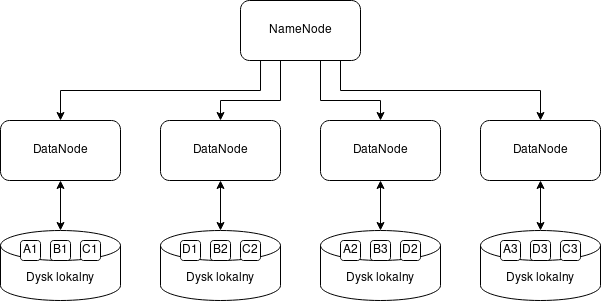
\includegraphics[width=0.7\textwidth]{./graf/HDFS.png}
      \caption{Schemat systemu plików HDFS}
      \label{fig:hdfs}
\end{figure}

\begin{figure}
      \centering
      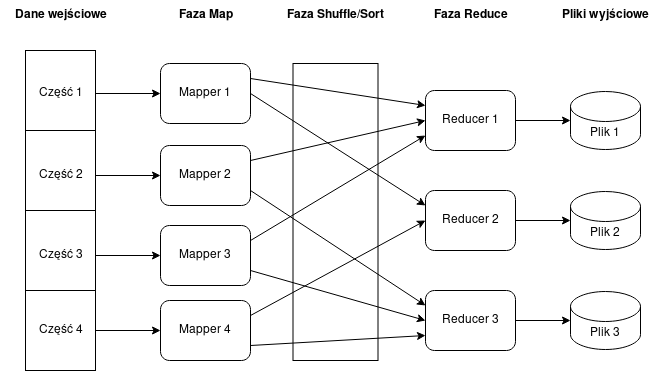
\includegraphics[width=0.8\textwidth]{./graf/MapReduce.png}
      \caption{Schemat przykładowego programu \english{MapReduce}}
      \label{fig:mapreduce}
\end{figure}

Klaster Apache Hadoop składa się z trzech głównych części:
\begin{enumerate}
      \item \english{Hadoop Distributed File System (HDFS)} –- rozproszony system plików dla
            platformy Hadoop. Pliki są dzielone na bloki (zazwyczaj o wielkości 128 MB lub 256 MB)
            i przechowywane w wielu egzemplarzach na różnych węzłach klastra (Rys. \ref{fig:hdfs}),
            zapewniając w ten sposób lokalność danych i odporność na awarie. System plików HDFS
            składa się z następujących komponentów:
            \begin{itemize}
                  \item NameNode –- węzeł zarządzający metadanymi i strukturą katalogów,
                  \item DataNode –- węzły przechowujące bloki danych i sumy kontrolne.
            \end{itemize}
      \item \english{MapReduce} –- domyślny model przetwarzania danych w Hadoop, wywodzący się
            z~systemów opracowanych przez Google. Na jego implementację w Apache Hadoop składają
            się następujące fazy (Rys. \ref{fig:mapreduce}):
            \begin{itemize}
                  \item \english{Map} –- przetwarzanie podzielonych danych wejściowych i utworzenie
                        par klucz-wartość, realizowane przez komponenty \english{Mapper},
                  \item \english{Shuffle/Sort} –- sortowanie par klucz-wartość i przesyłanie ich między węzłami,
                  \item \english{Reduce} –- łączenie wartości o tym samym kluczu, realizowane przez
                        komponenty o nazwie \english{Reducer}.
            \end{itemize}
            Użytkownicy definiują etapy \english{Map} i \english{Reduce}, natomiast etap sortowania
            dostarczany jest przez Hadoop.
      \item \english{Yet Another Resource Negotiator (YARN)} –- menedżer zasobów i system przydzielania
            zadań dla Hadoop, który pozwala wielu aplikacjom współdzielić zasoby w~jednym środowisku.
            Składa się z trzech typów węzłów:
            \begin{itemize}
                  \item ResourceManager –- odpowiedzialny za alokację zasobów w klastrze,
                  \item ApplicationMaster –- zarządza pojedynczym zadaniem oraz śledzi jego postęp,
                  \item NodeManager -– zarządza pojedynczym węzłem wykonawczym, komunikuje informacje
                        o dostępnych zasobach.
            \end{itemize}
\end{enumerate}

Choć implementacje faz \english{Map} i \english{Reduce} są pisane głównie w języku Java, to
narzędzie \english{Hadoop Streaming} pozwala na użycie dowolnego programu, który komunikuje się
za pomocą standardowych strumieni wejścia/wyjścia. Wskutek tego możliwe jest tworzenie
komponentów \english{Mapper} oraz \english{Reducer} w dowolnym języku programowania.

Hadoop i model MapReduce zostały zaprojektowane głównie dla aplikacji wsadowych, co oznacza,
że są lepiej przystosowane do przetwarzania dużych, zamkniętych zbiorów danych niż do ciągłego
przetwarzania strumieniowego lub iteracyjnego.

\section{Apache Spark}

Apache Spark to otwarta platforma do rozproszonego przetwarzania dużych zbiorów danych,
która oferuje wsparcie dla programów wsadowych, obróbki danych w czasie rzeczywistym,
interaktywnej analizy danych i uczenia maszynowego. Spark został opracowany w celu pokonania
ograniczeń wynikających z szybkości dysków twardych.

Platforma Spark jest oparta o struktury danych \english{Resilient Distributed Dataset (RDD)}.
Są to obiekty przechowywane w pamięci węzłów klastra w wielu egzemplarzach, które mogą być
przetwarzane równolegle. Ich użycie pozwala na nawet stukrotne przyspieszenie w porównaniu z
systemami opartymi o Apache Hadoop, zachowując jednocześnie wysoką odporność na awarie \cite{big-data-3}.

Spark zapewnia wsparcie dla wielu źródeł danych. Są to między innymi HDFS, bazy Apache
Cassandra, relacyjne bazy danych SQL i źródła Amazon S3. System ten wspiera też wiele
języków programowania, są to na przykład Scala, Python, Java oraz R.

Klaster Apache Spark może działać niezależnie, w połączeniu z systemem plików HDFS lub
z innymi systemami zarządzania klastrem:
\begin{itemize}
      \item YARN -- menedżer zasobów dla platformy Apache Hadoop,
      \item Apache Mesos -- menedżer klastra zgodny z Hadoop oraz Spark,
      \item Kubernetes -- platforma do wdrażania i skalowania aplikacji kontenerowych.
\end{itemize}

\subsubsection*{Spark SQL}

Moduł Spark SQL umożliwia przetwarzanie danych w formacie tabelarycznym przy użyciu języka
SQL \cite{spark-sql}. Spark SQL zapewnia też dostęp do danych z Apache Hive i interfejsy
dostępu do relacyjnych baz danych (JDBC oraz ODBC), co ułatwia integrację z~istniejącymi
aplikacjami.

%TC:ignore
\begin{lstlisting}[
    language=Java,
    label=lst:spark-sql,
    caption={Przykładowy program wykorzystujący moduł Spark SQL.}
]
public class SparkSQLExample {

    public static void main(String[] args) {
        SparkSession spark = SparkSession.builder()
            .appName("Spark SQL w Javie")
            .master("local")
            .getOrCreate();

        // Wczytanie danych z pliku CSV
        Dataset<Row> df = spark.read()
            .option("header", "true")
            .option("inferSchema", "true")
            .csv("osoby.csv");

        // Utworzenie widoku tymczasowego
        df.createOrReplaceTempView("osoby");

        // Wykonanie zapytania SQL
        Dataset<Row> wynik = spark.sql(
            "SELECT imie, wiek FROM osoby WHERE wiek > 25"
        );
        wynik.show(); // Pokazanie wyniku w konsoli
        spark.stop();
    }
}
\end{lstlisting}
%TC:endignore

Jednym z kluczowych elementów Spark SQL jest DataFrame, czyli rozproszona kolekcja danych
zorganizowana w kolumny. DataFrame można przyrównać do tabeli w relacyjnej bazie danych,
ponieważ wspiera on wykonywanie operacji takich jak wybieranie, filtrowanie czy agregacja.

Wraz z DataFrame pojawiły się także struktury Dataset, które łączą zalety RDD i~DataFrame,
oferując zarówno typowanie statyczne, jak i operacje na poziomie kolumn. Dataset to kolekcja
obiektów określonego typu, co oznacza, że błędy związane z typami mogą być wykrywane w czasie
kompilacji, a nie tylko podczas wykonania.

Statyczne typowanie zapewnia większe bezpieczeństwo i pewność podczas pisania kodu w
porównaniu do operacji wykonywanych na DataFrame'ach, które są typowane dynamicznie.
Przykład wykorzystania Dataset pokazano na listingu \ref{lst:spark-sql}.

Catalyst to optymalizator używany przez Spark SQL, który optymalizuje zapytania SQL na dwóch
poziomach: najpierw na poziomie planu logicznego, następnie na poziomie planu fizycznego
\cite{spark-sql-catalyst}. Plan logiczny opisuje tylko etapy potrzebne do obliczenia wyniku,
nie uwzględniając jednak struktury klastra. Informacje te posiada plan fizyczny, który składa
się z optymalnych struktur RDD i algorytmów, dopasowanych do konkretnego klastra Spark.

Ważną cechą optymalizatora Catalyst jest oddzielenie optymalizacji od logiki zapytania. Taki
podział ułatwia wdrażanie aktualizacji i modyfikacji, a same optymalizacje mogą być używane
w wielu zapytaniach jednocześnie, co wpływa korzystnie na długoterminowe utrzymanie całego
systemu. Co więcej, optymalizacje są dobierane dynamicznie, dzięki czemu to samo zapytanie
może być wykonywane optymalnie na klastrach o różnych rozmiarach, topologiach czy
dostępnych zasobach.

\section{Architektura CUDA}

CUDA (ang. \english{Compute Unified Device Architecture}) to jedna z najbardziej popularnych
równoległych architektur dla procesorów graficznych, opracowana przez firmę NVIDIA.

Architektura CUDA realizuje model SIMT \cite{computer-arch} (ang. \english{Single Instruction, Multiple Threads},
jedna instrukcja -- wiele wątków), który łączy zalety wielowątkowości i instrukcji wektorowych.
Podstawowym elementem tego modelu jest wątek CUDA, czyli najmniejsza jednostka obliczeń, która
może być niezależnie zaplanowana do wykonania przez procesor.

Podobnie jak w modelu SIMD (ang. \english{Single Instruction, Multiple Data}, jedna instrukcja -- wiele danych),
w architekturze CUDA instrukcje są wykonywane równolegle na wielu danych. Z drugiej strony,
w modelu SIMT każdy wątek posiada własny kontekst, składający się ze stosu i rejestrów.

\begin{figure}
      \centering
      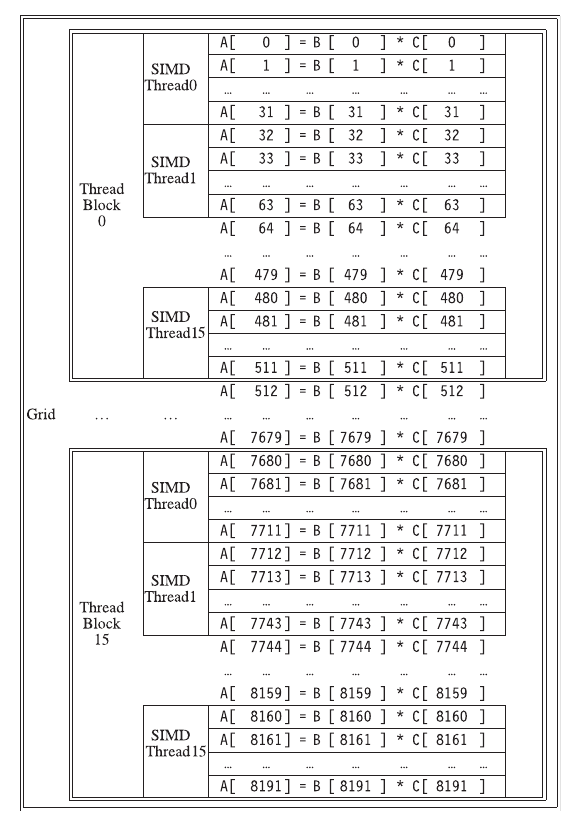
\includegraphics[width=0.8\textwidth]{graf/CUDA-Grid.png}
      \caption {
            Podział przykładowego programu CUDA na siatkę (ang. \english{grid}),
            bloki wątków (ang. \english{thread block}) i wątki CUDA (ang. \english{thread}).
            \cite{computer-arch}
      }
      \medskip \small
      Program mnoży elementy tablic B i C, wynik jest zapisywany do tablicy A.
      \label{fig:cuda-grid}
\end{figure}

\newpage
Wątki CUDA są zorganizowane w grupy zwane blokami (Rys. \ref{fig:cuda-grid}), w których obrębie
mogą wymieniać się danymi przez pamięć współdzieloną i synchronizować się za pomocą
barier. Zarówno bloki wątków, jak i siatki składające się z tych bloków mogą być organizowane na
różne sposoby przy użyciu struktur jedno-, dwu- lub trójwymiarowych. Ta elastyczność pomaga w
tworzeniu wydajnych programów, które pozostają proste i łatwe w utrzymaniu.

W architekturze CUDA hierarchia pamięci odgrywa kluczową rolę w efektywnym wykorzystaniu
układów graficznych. Model programowania CUDA udostępnia następujące rodzaje pamięci:
\begin{itemize}
      \item rejestry -- najszybsza dostępna pamięć, używana przez pojedyncze wątki, przechowuje
            zmienne lokalne. Liczba dostępnych rejestrów jest ograniczona i zależy od generacji procesora CUDA.
      \item pamięć współdzielona -- szybka pamięć procesora, dostępna dla wątków w obrębie jednego bloku.
            Ma ograniczoną pojemność, ale dostęp do niej jest znacznie szybszy niż do pamięci globalnej.
            Aby zapewnić maksymalną wydajność, ważne jest unikanie konfliktów banków tej pamięci.
      \item pamięć globalna -- zewnętrzna pamięć procesora, dostępna dla wszystkich bloków i~wątków.
            Jest największa pod względem pojemności, ale jednocześnie ma najwyższe opóźnienia dostępu.
            Wspiera dostępy łączone, które znacznie przyspieszają operacje czytania oraz zapisu.
      \item pamięć stałych -- specjalny segment pamięci globalnej o ograniczonej pojemności, który
            jest przechowywany w pamięci podręcznej. Przeznaczony dla parametrów funkcji oraz danych,
            które nie zmieniają się podczas wykonywania programu.
      \item pamięć tekstur -- zoptymalizowana dla specyficznych wzorców dostępu, typowych dla programów
            związanych z grafiką komputerową. Dane podlegają przechowywaniu w~pamięci podręcznej procesora.
      \item pamięć lokalna -- segment pamięci globalnej, który jest używany do przechowywania zmiennych
            lokalnych wątku, gdy przekroczy on dostępną liczbę rejestrów. Charakteryzuje się większymi
            opóźnieniami od pamięci współdzielonej, ponieważ jest fizycznie przechowywana w zewnętrznej pamięci DRAM.
\end{itemize}

Układy graficzne firmy NVIDIA oferują jednakowy model programowania i wykorzystują wspólny pakiet narzędzi
programistycznych, co ułatwia tworzenie przenośnych programów. Częścią modelu programowania jest język
programowania CUDA \cite{cuda-by-example}, który jest w istocie rozszerzeniem języka C++ o hierarchiczny
model pamięci urządzenia, funkcje do synchronizacji wątków, typy wektorowe oraz możliwość definiowania
funkcji wykonywanych na procesorze graficznym, określanych też jako \english{kernel}.

Kod napisany w języku CUDA może być kompilowany do przenośnego kodu pośredniego PTX
(ang. \english{Parallel Thread Execution}), co umożliwia jego późniejszą optymalizację i wykonanie
na urządzeniach o różnych wersjach architektury CUDA.

Dzięki szerokiej dostępności bibliotek, programy CUDA mogą być wywoływane także z poziomu
innych języków, takich jak Python, Java, MATLAB oraz Rust. Niektóre narzędzia, takie jak CudaPy
dla języka Python, pozwalają też na automatyczne tłumaczenie funkcji na kod CUDA.

\section{Standard OpenCL}

OpenCL (ang. \english{Open Computing Language}) to otwarty standard umożliwiający tworzenie programów
wykorzystujących akcelerację sprzętową, w tym różnorodne kombinacje procesorów głównych, graficznych oraz
innych akceleratorów \cite{opencl}.

W porównaniu z technologią CUDA, której rozwojem kieruje NVIDIA, OpenCL został stworzony przez konsorcjum
Khronos Group określające jedynie specyfikację interfejsów. Dostarczenie odpowiednich sterowników i
implementacji OpenCL jest z kolei zadaniem należącym do producenta sprzętu.

Ze względu na otwartość tego standardu, OpenCL umożliwia pisanie kodu, który może być łatwo przenoszony i
dostosowywany do różnych architektur i platform sprzętowych. Pozwala to na większą elastyczność w projektowaniu
systemów prowadzących obliczenia.

Jednostka obliczeń (ang. \english{work-item}), odpowiadająca wątkowi w modelu CUDA, stanowi najmniejsze
możliwą do zaplanowania i wykonania zadanie. Tak jak w modelu CUDA, jednostki obliczeń mogą być organizowane
w grupy robocze (ang. \english{workgroup}), które są odpowiednikami bloków wątków. Komunikacja w obrębie
grupy roboczej jest realizowana poprzez pamięć lokalną. Mechanizmy synchronizacji, takie jak bariery, pozwalają
na koordynację wykonania jednostek w ramach grupy roboczej.

OpenCL oferuje programistom złożony, ale jednakowy dla wszystkich urządzeń model pamięci. Jego hierarchiczna
struktura składa się z następujących elementów:
\begin{itemize}
      \item pamięć prywatna -- pamięć dostępna tylko dla jednej jednostki obliczeń. Dane w pamięci prywatnej nie
            są dostępne dla innych jednostek wykonawczych. Zazwyczaj jest używana do przechowywania zmiennych
            lokalnych w funkcjach. Jest to ekwiwalent pamięci lokalnej w CUDA.
      \item pamięć lokalna -- dostępna dla wszystkich jednostek obliczeń w obrębie jednej grupy roboczej. Jest szybsza
            niż pamięć globalna i idealnie nadaje się do przechowywania tymczasowych danych. Podobna do pamięci
            współdzielonej w modelu CUDA. \newpage
      \item pamięć globalna -- pamięć dostępna dla wszystkich jednostek obliczeń w~obrębie kernela. Ze względu
            na jej globalny charakter, dostęp do niej może być wolniejszy w~porównaniu z innymi rodzajami pamięci,
            dlatego jej użycie powinno być ograniczane. Jest odpowiednikiem pamięci globalnej w CUDA.
      \item pamięć stałych -- specjalny segment pamięci globalnej, który może być odczytywany przez jednostki
            obliczeń. Na niektórych urządzeniach jest to część pamięci podręcznej. Odpowiednik pamięci stałych w CUDA.
\end{itemize}

Ze względu na konieczność zapewnienia wsparcia dla różnych typów procesorów, model pamięci OpenCL nie
zawiera pamięci tekstur, pozwalającej na optymalizację wzorców dostępu typowych dla aplikacji grafiki komputerowej.

Oprócz modelu obliczeń i pamięci, OpenCL opisuje też języki programowania przeznaczone dla
akceleratorów. Są to języki oparte o standardy C99, C++14 i C++17, rozszerzające je o funkcje
związane z zarządzaniem pamięcią, synchronizacją jednostek obliczeń oraz operacjami wektorowymi.

Podobnie jak w przypadku języka CUDA, kod OpenCL może być kompilowany do reprezentacji pośredniej.
W przypadku OpenCL jest to SPIR (ang. \english{Standard Portable Intermediate Representation}),
który przed wykonaniem programu jest optymalizowany dla architektury konkretnego urządzenia.

\section{Klastry oparte o minikomputery jednopłytkowe}

Klastry obliczeniowe zbudowane z komputerów jednopłytkowych cechują się dużą skalowalnością.
Dobrym przykładem są systemy zbudowane przez firmy Balena i Oracle, które służą głównie jako
demonstratory technologii do rozproszonego przechowywania danych i~zarządzania serwerami,
składają się zatem z setek lub nawet tysięcy węzłów.

Klaster Beast v2 został skonstruowany przez firmę Balena jako następca wcześniejszej wersji,
Beast v1. Składa się on ze 144 minikomputerów Raspberry Pi 3B, połączonych siecią Gigabit
Ethernet. Konstrukcja ukazana na rysunku \ref{fig:balena-cluster} osiąga wysokość 2 metrów
i~masę około 150 kilogramów.

Klaster był pierwotnie przeznaczony do testowania i demonstracji oprogramowania resin.io,
a ostatecznie został wysłany do klienta, który sponsorował jego budowę. Wkrótce potem
rozpoczęto projektowanie kolejnej iteracji, nazwanej "Beast v3", która ma na celu dalsze
zwiększenie modułowości, gęstości i łatwości montażu \cite{balena-cluster}.
\newpage

\begin{figure}
      \centering
      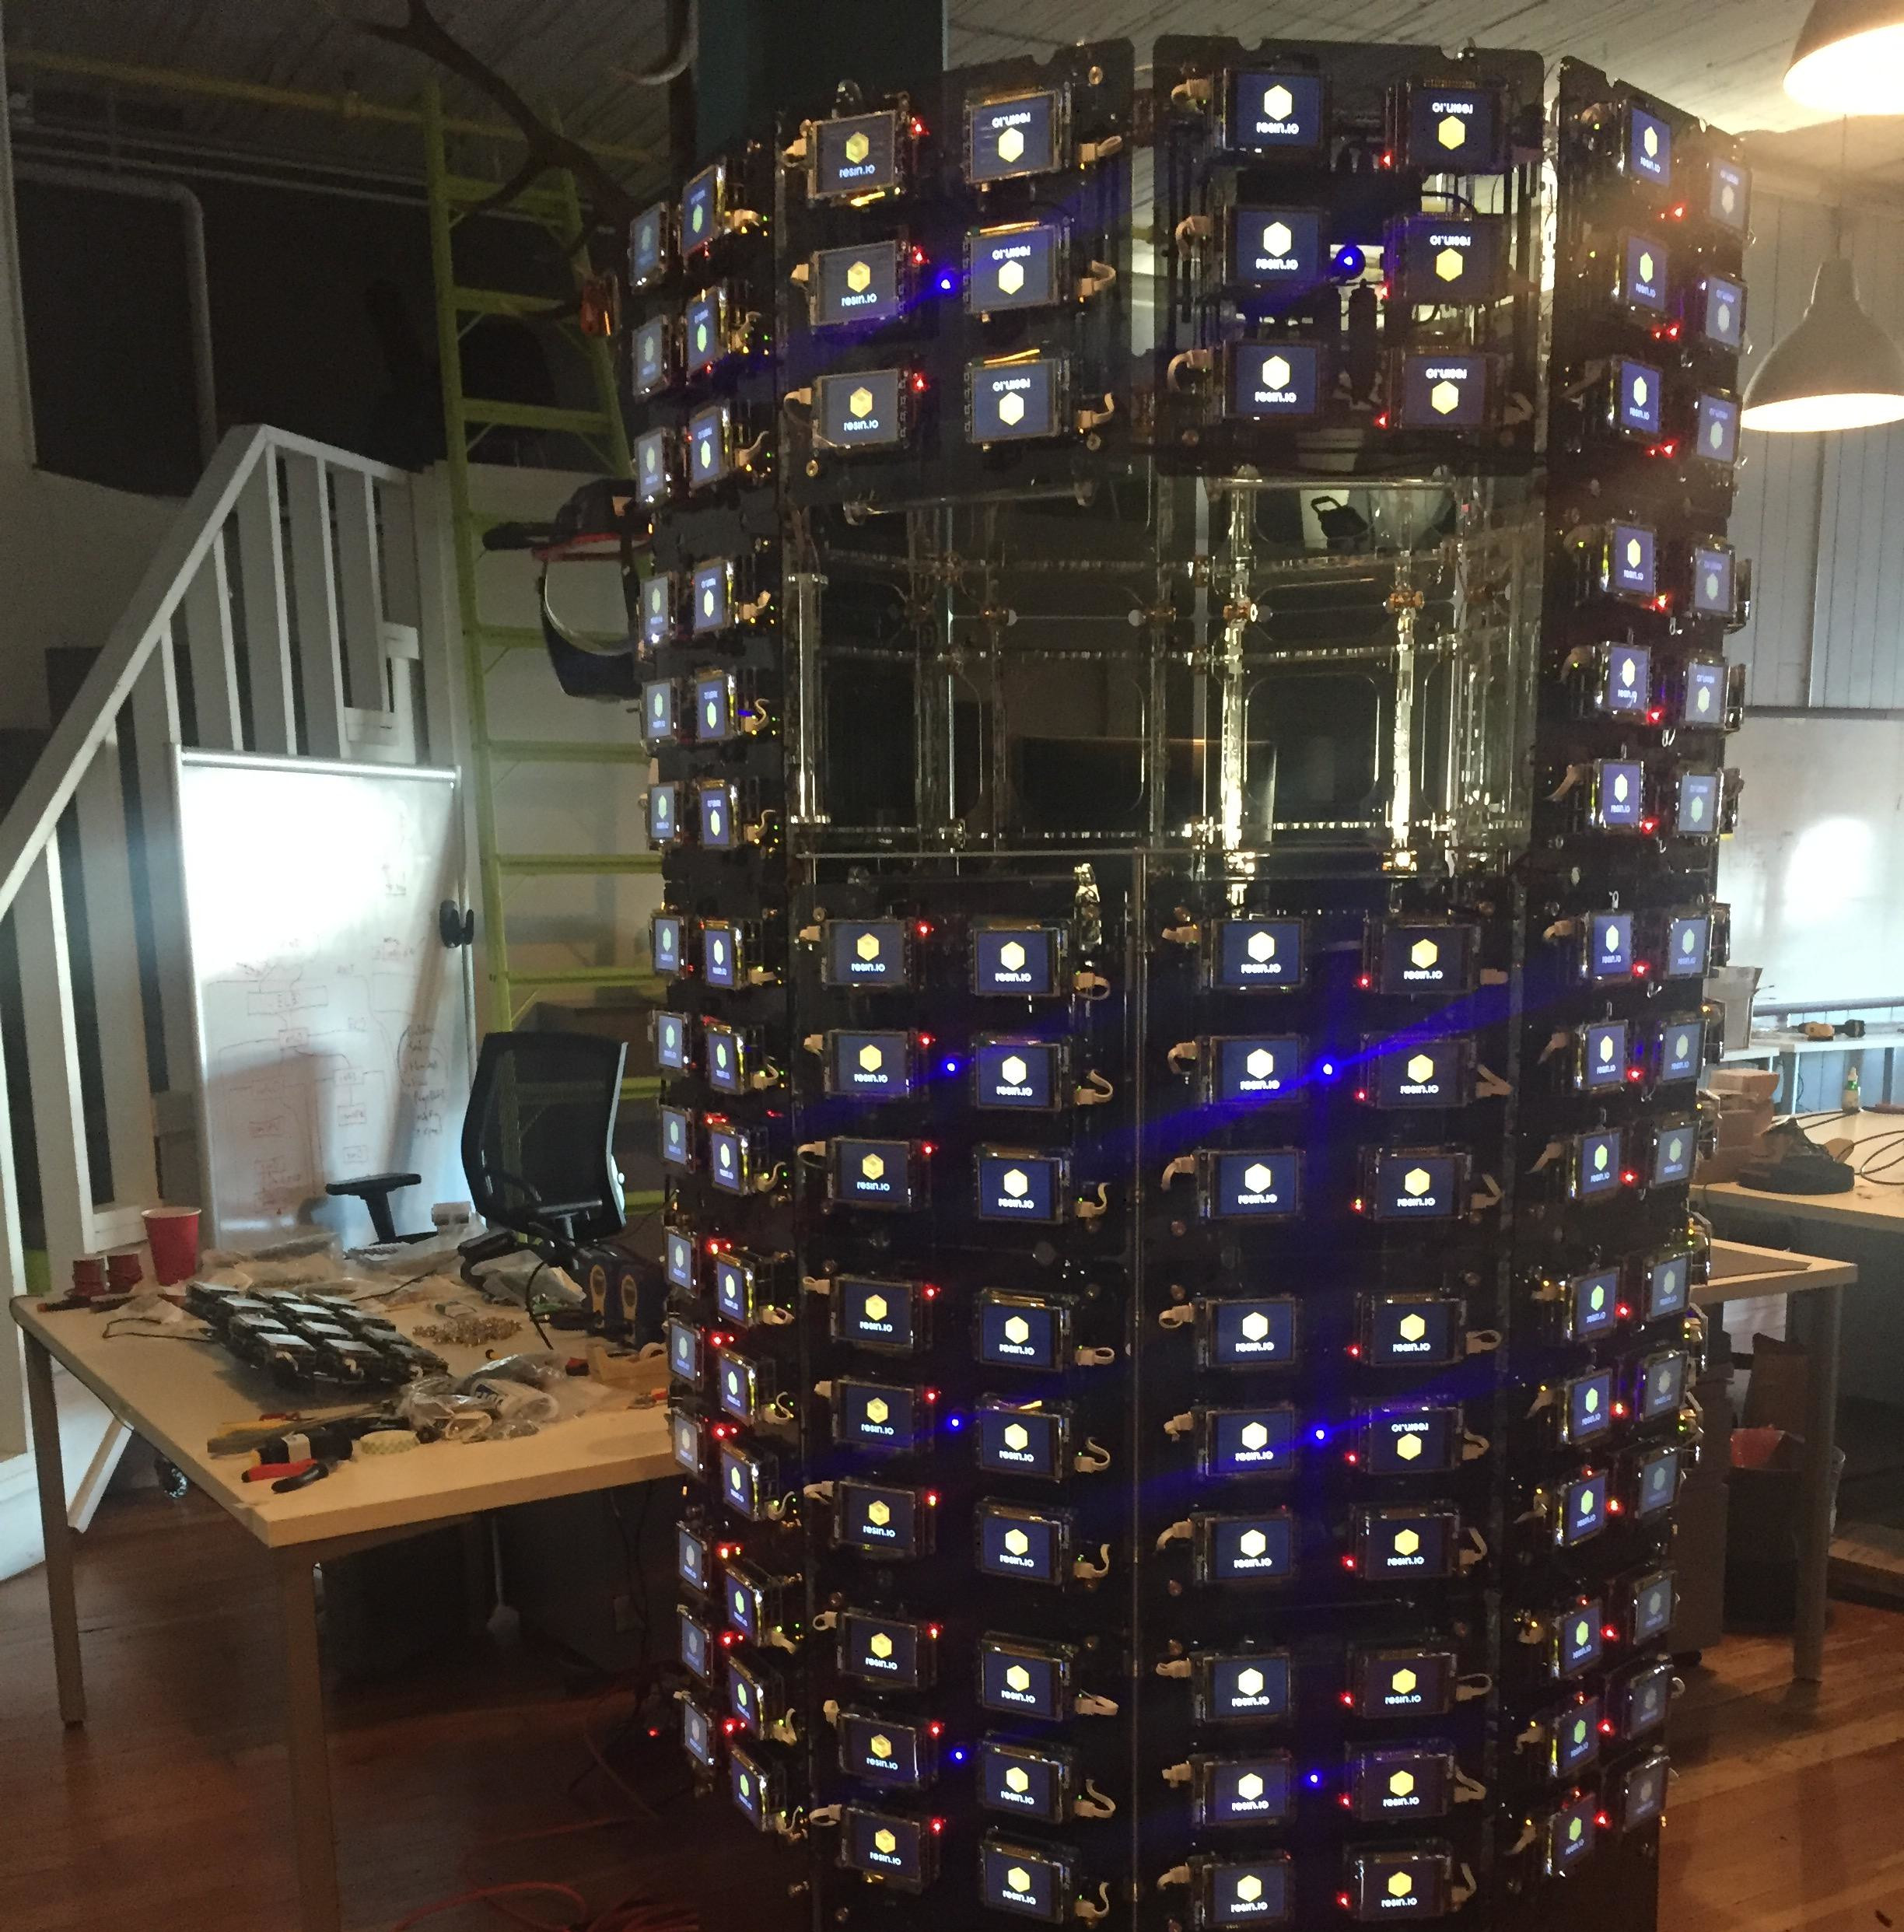
\includegraphics[width=0.8\textwidth]{graf/Balena.jpg}
      \caption {
            Klaster Beast v2. \cite{balena-cluster}
      }
      \label{fig:balena-cluster}
\end{figure}

System firmy Oracle, nazwany \english{Raspberry Pi Supercomputer}, został zaprezentowany po raz
pierwszy na targach OpenWorld 2019 (Rys. \ref{fig:oracle-cluster}). Składa się on z 1060
minikomputerów Raspberry Pi 3B+ umieszczonych w szafach 2U, gdzie każda półka mieści 21 węzłów.
Węzły zostały połączone za pomocą sieci w standardzie Gigabit Ethernet.

Komputery Raspberry Pi zostały umieszczone w obudowach wykonanych w technologii druku 3D.
Zasilanie węzłów jest zapewniane przez zasilacze USB, które zostały wybrane ze względu na
mniejszy koszt i większą sprawność w porównaniu do zasilania przez interfejsy Ethernet
(ang. \english{Power over Ethernet, PoE}). Wdrożenie Oracle Linux zostało przeprowadzone
za pomocą centralnego serwera rozruchowego \cite{oracle-cluster-1}.

Przedstawiony klaster pokazał możliwości dystrybucji Oracle Linux, języka programowania Java
oraz bazy danych Oracle w kontekście integracji powszechnie dostępnych komponentów, takich jak
Raspberry Pi, w klastry obliczeniowe dużego formatu \cite{oracle-cluster-2}.
\newpage

\begin{figure}
      \centering
      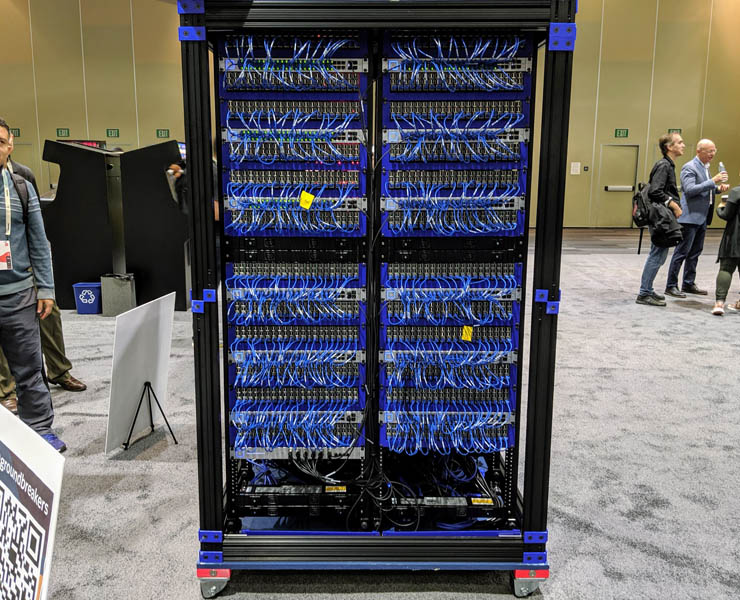
\includegraphics[width=0.9\textwidth]{graf/Oracle.jpg}
      \caption {Klaster Raspberry Pi Supercomputer firmy Oracle. \cite{oracle-cluster-1}}
      \label{fig:oracle-cluster}
\end{figure}

Artykuł autorstwa A. Neto, J. Neto i E. Moreno \cite{rpi-cluster-1} opisuje klaster
\english{Big Data} wykorzystujący platformę Apache Hadoop i 9 minikomputerów Raspberry Pi 4B.
Minikomputery wykorzystują karty pamięci microSD jako dysk systemowy, a komunikacja
między węzłami klastra realizowana jest przez sieć Ethernet. Przepustowość tej sieci
nie została określona przez autorów.

Oprócz opisu użytego sprzętu i oprogramowania artykuł zawiera również kompletny poradnik,
który przedstawia proces instalacji, konfiguracji oraz testowania wydajności. W artykule
są też załączone informacje na temat narzędzi wykorzystanych do testów, metodologii
testowania, użytych danych wejściowych i konfiguracji klastra.

Aby ocenić funkcjonalność i wydajność skonstruowanego klastra, autorzy wykorzystali narzędzia
TeraSort oraz TestDFSIO, które stanowią część oficjalnej dystrybucji Apache Hadoop.
Dla każdej liczby węzłów wykonawczych (2, 4, 8) zbadano wydajność dla 4 rodzajów danych
wejściowych. Wyniki zostały porównane pod kątem przyrostu wydajności w zależności
od liczby węzłów, nie przeprowadzono porównania z innymi klastrami. \newpage

Klaster opisany przez E. Lee, H. Oh oraz D. Park \cite{rpi-cluster-2} składa się z 6
minikomputerów Raspberry Pi 4B. W porównaniu do poprzedniego artykułu opisane jest
użycie platformy obliczeniowej Apache Spark. Węzły klastra zostały połączone siecią
Gigabit Ethernet.

Wydajność została zbadana nie tylko pod kątem liczby węzłów, ale także z uwzględnieniem
dysków systemowych o różnej wydajności. W przytoczonym badaniu są to karty pamięci
microSD o klasach szybkości UHS-1, UHS-3 oraz UFS.

Szerszy jest też zestaw przetestowanych programów -- są to TestDFSIO, Wordcount, TeraGen,
TeraSort oraz QuasiMonteCarlo. Wydajność klastra została porównana z klastrem Raspberry Pi
poprzedniej generacji oraz pojedynczym komputerem klasy PC.

W artykule poruszono też inne czynniki wpływające na wydajność klastra, są to między innymi
mechanizmy sum kontrolnych w HDFS, topologia rozproszonego systemu plików oraz chłodzenie
procesora. Przeprowadzona analiza opłacalności wykazała, że klaster Raspberry Pi złożony
z 7 węzłów byłby konkurencyjny z komputerem PC pod względem wydajności przy jednoczesnej
redukcji zużycia prądu.
 % [Analiza tematu]
\chapter{Budowa klastra obliczeniowego} \label{ch:budowa-klastra}

W przeszłości głównym zastosowaniem procesorów graficznych było przyspieszanie renderowania
grafiki, głównie w kontekście gier i graficznych interfejsów użytkownika. Wraz z ewolucją
tych układów, rozwinęła się ich zdolność do równoczesnego przetwarzania bardzo dużej liczby
wątków, co pozwala na znaczące przyspieszenie innych aplikacji o~wysokim stopniu równoległości.

Dobrym tego przykładem są nowoczesne układy graficzne, które udostępniają setki, a nawet
tysiące rdzeni dla obliczeń ogólnego przeznaczenia. Dzięki temu są stosunkowo tanim
narzędziem do równoległego przetwarzania danych na wielką skalę \cite{computer-arch}.

Aby zwiększyć wydajność proponowanego klastra względem istniejących rozwiązań, minikomputery
jednopłytkowe będące węzłami wykonawczymi powinny wspierać obliczenia ogólnego przeznaczenia
na układach graficznych (ang. \english{General-Purpose Compute on Graphics Processing Units, GPGPU}).
Szczególnie ważne w tym przypadku jest wsparcie dla popularnych narzędzi do programowania
GPGPU, takich jak CUDA oraz OpenCL.

Aby zapewnić efektywne przechowywanie, transfer i przetwarzanie danych, węzły klastra
powinny posiadać też:
\begin{itemize}
	\item dużą ilość szybkiej pamięci RAM,
	\item szybkie interfejsy dla pamięci trwałej (dyski HDD lub SSD),
	\item karty sieciowe o dużej przepustowości.
\end{itemize}

\section{Porównanie minikomputerów z akceleracją GPU}

Model Raspberry Pi 4, wydany w 2019 roku, przyniósł znaczące ulepszenia pod względem wydajności
w porównaniu do swoich poprzedników. Choć szybsze interfejsy sieciowe, większa ilość pamięci RAM
(nawet do 8 GB) oraz interfejsy USB 3.0 pozwoliły na znaczne zwiększenie wydajności w obliczeniach
\english{Big Data} \cite{rpi-cluster-2}, to brak wsparcia dla technologii CUDA i OpenCL czyni ten
model niewystarczającą podstawą dla węzłów wykonawczych.

Popularnym przedstawicielem minikomputerów jednopłytkowych jest też Intel NUC. Jednostki te
oferują wydajne procesory x86, wbudowane układy graficzne, obsługę szybkich dysków i dużą
rozszerzalność. Komputery NUC są dostępne zarówno w formie gotowych urządzeń, jak i zestawów
do samodzielnego złożenia, co pozwala na dostosowanie ich do konkretnych potrzeb użytkownika.
Najnowsze produkty z tej linii oferują wsparcie dla technologii OpenCL oraz akceleratory
sieci neuronowych, lecz nie wspierają technologii CUDA \cite{nuc-list}.

Nvidia Jetson to kolejna rodzina minikomputerów z akceleracją GPU, początkowo przeznaczona
przede wszystkim do rozwoju aplikacji graficznych 3D. Wkrótce komputery z tej serii stały
się też popularnym narzędziem do prototypowania aplikacji wizji komputerowej, uczenia
maszynowego i Internetu rzeczy.

Swoją popularność zawdzięczają wsparciu technologii CUDA i OpenCL, stosunkowo niskiemu
kosztowi, małym wymiarom oraz obszernemu pakietowi narzędzi Nvidia JetPack SDK.
Biorąc pod uwagę te zalety, do budowy klastra wybrano model Jetson Nano.

Zestaw Jetson Nano Developer Kit wyróżnia się \cite{jetson-spec}:
\begin{itemize}
	\item 128-rdzeniowym procesorem graficznym o maksymalnej wydajności 472 GFLOPS,
	      wspierającym technologie CUDA oraz (nieoficjalnie) OpenCL,
	\item czterordzeniowym procesorem ARM Cortex-A57 o taktowaniu 1.43GHz,
	\item 4 GiB pamięci RAM w technologii LPDDR4, o łącznej przepustowości 25.6 GB/s,
	\item kartą sieciową obsługującą standard Gigabit Ethernet,
	\item obsługą kart pamięci SD, pamięci Flash eMMC i dysków zewnętrznych USB 3 o przepustowości do 5 Gbit/s,
	\item konfigurowalnym poborem mocy (od 5 do 10W),
	\item zasilaniem poprzez port microUSB.
\end{itemize}

\section{Sprzęt i oprogramowanie}

\begin{figure}[h]
	\centering
	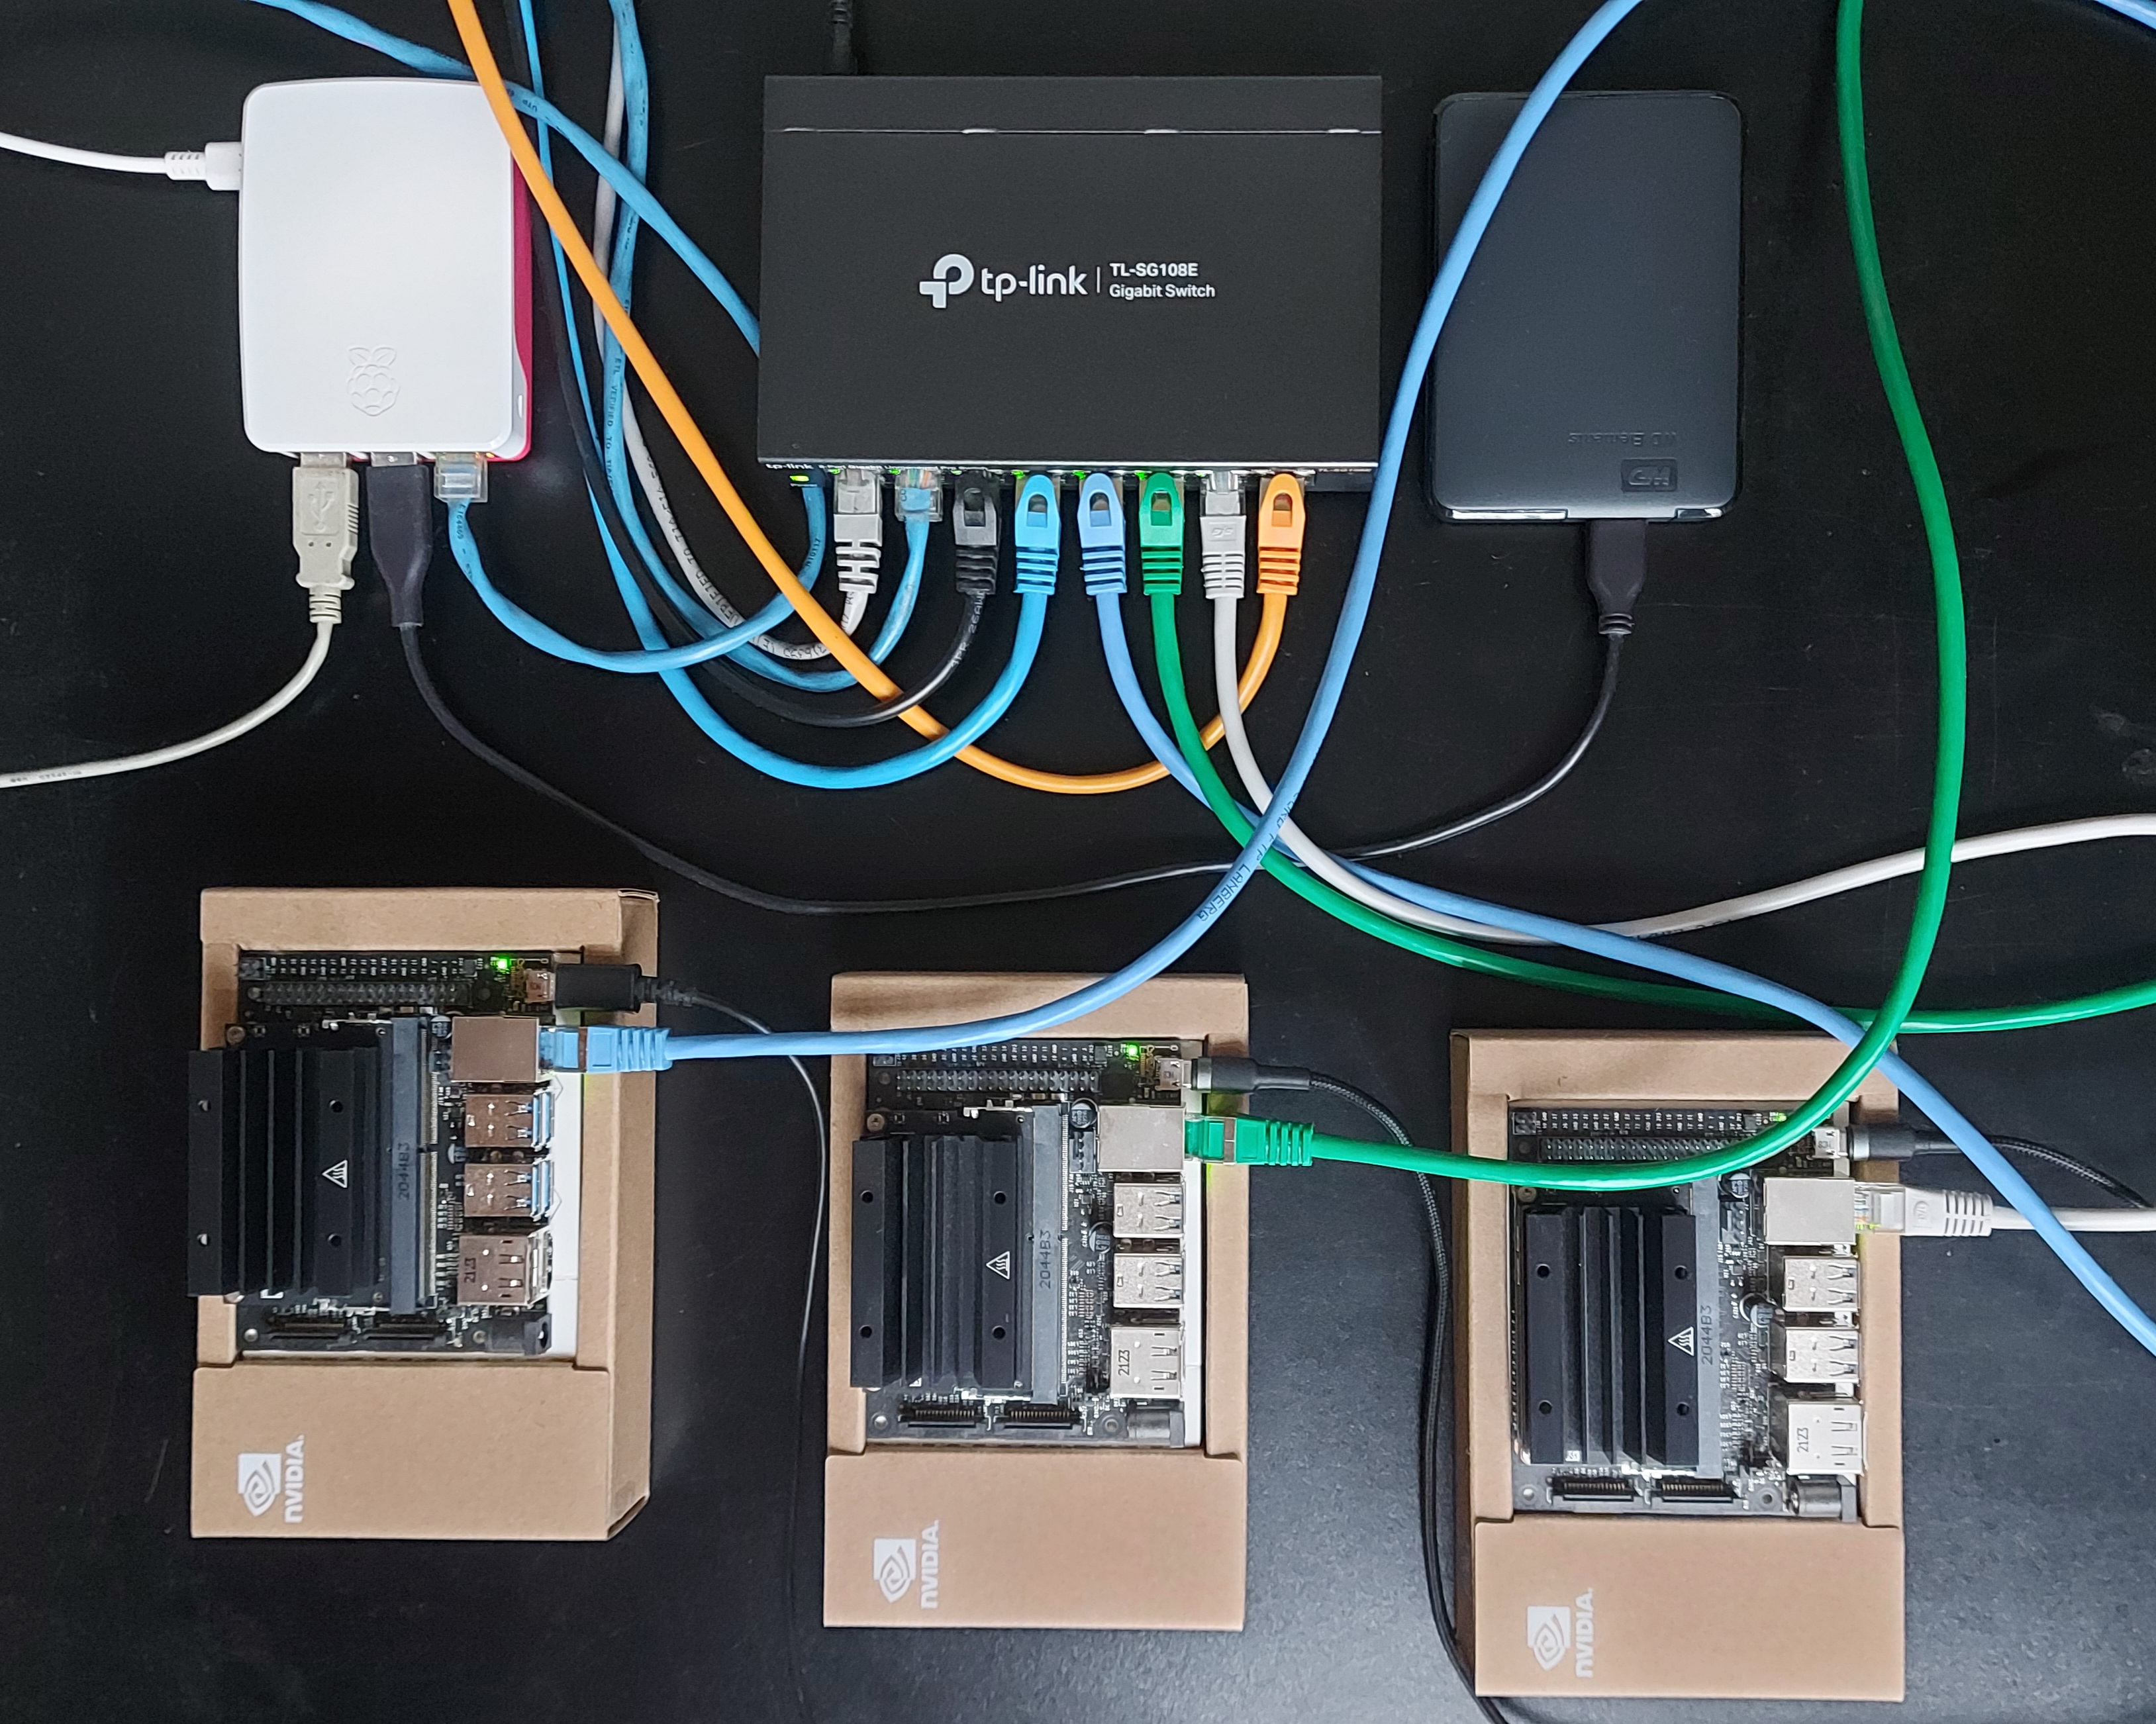
\includegraphics[width=0.7\textwidth]{graf/Cluster-picture.jpg}
	\caption{Klaster minikomputerów zbudowany na potrzeby pracy.}
	\medskip \small
	U góry, kolejno od lewej strony: minikomputer Raspberry Pi 4B, przełącznik sieciowy
	TP-Link oraz dysk zewnętrzny. Na dole widoczne minikomputery Nvidia Jetson Nano.
	\label{pic:cluster-photo}
\end{figure}

Klaster przedstawiony na fotografii \ref{pic:cluster-photo} składa się z czterech węzłów, w tym
jednego węzła nadrzędnego i trzech węzłów wykonawczych. Funkcję węzła nadrzędnego pełni
minikomputer Raspberry Pi 4B w wersji z 2 GB pamięci RAM, który został dodatkowo wyposażony w
dysk twardy USB 3.0 o pojemności 1 TB. Zasilanie minikomputera zapewniane jest przez
zasilacz USB-C dedykowany dla Raspberry Pi.
\newpage

Węzły wykonawcze klastra to minikomputery Nvidia Jetson Nano w wersji z 4 GB pamięci RAM, które
zasilane są przez ładowarkę USB firmy Aukey. Wybrana ładowarka dostarcza maksymalnie 12 W na
każdy z czterech portów, przez co każdy moduł Jetson Nano jest w stanie w pełni wykorzystać
limit poboru mocy.

Rolę dysków dla minikomputerów Jetson Nano pełnią karty microSD SanDisk o~pojemności 16 GB i
klasie szybkości UHS-1. Gwarantują one minimalną szybkość zapisu 10 MB/s i maksymalną
szybkość odczytu do 120 MB/s.

Zgodnie ze schematem przedstawionym na rysunku \ref{fig:cluster-network}, wszystkie węzły
klastra są połączone siecią Gigabit Ethernet poprzez przełącznik sieciowy TP-Link.
Aby ułatwić konfigurację klastra, adresy IP minikomputerów zostały przydzielone statycznie.

\begin{figure}[h]
	\centering
	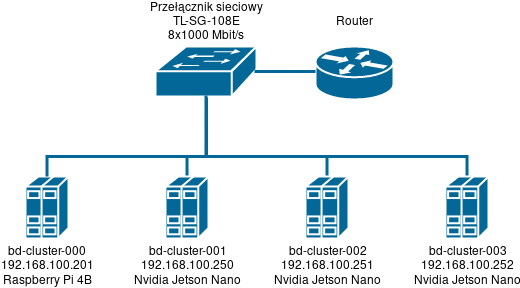
\includegraphics[width=0.6\textwidth]{graf/Cluster-network.png}
	\caption{Schemat sieci komputerowej łączącej węzły klastra.}
	\label{fig:cluster-network}
\end{figure}

Węzeł nadrzędny klastra działa pod kontrolą systemu operacyjnego Ubuntu Server LTS w wersji 20.04.
W przypadku węzłów wykonawczych wykorzystywana jest dystrywbucja Nvidia Jetson Linux w wersji
R32.7.3 (Tab. \ref{tab:software}), która dostarcza sterowniki, biblioteki i narzędzia potrzebne do
rozwoju aplikacji CUDA na platformie Jetson.

Ze względu na brak oficjalnego wsparcia OpenCL dla minikomputera Jetson Nano wykorzystano
otwartą implementację PoCL. Dzięki zastosowaniu projektu LLVM do generacji kodu maszynowego
obsługuje ona wiele architektur, w tym x86, ARM oraz CUDA. Wersja PoCL zawarta w systemie
Jetson Linux domyślnie nie zawiera wsparcia dla architektury CUDA, dlatego też na potrzeby
pracy przygotowano własną kompilację.

Na klastrze zostały zainstalowane platformy Apache Hadoop oraz Apache Spark, a~także wymagane do
ich uruchomienia środowiska OpenJDK 11 i Scala 2.13.

%TC:ignore
\begin{table}[h]
	\centering
	\caption{Wykaz oprogramowania wykorzystanego w badaniach.}
	\begin{tabular}{ | p{7cm} | p{2cm} | p{3cm} | }
		\hline
		Nazwa programu lub biblioteki & Wersja   & Data wydania \\
		\hline
		Nvidia Jetson Linux           & R32.7.3  & 2022-11-22   \\
		Ubuntu Server                 & 20.04.6  & 2023-03-23   \\
		OpenJDK                       & 11.0.19  & 2023-04-18   \\
		Scala                         & 2.13.11  & 2023-06-07   \\
		CUDA Toolkit                  & 10.2.460 & 2021-03-02   \\
		PoCL                          & 3.0      & 2022-06-10   \\
		Apache Hadoop                 & 3.3.5    & 2023-03-22   \\
		Apache Spark                  & 3.4.0    & 2023-04-13   \\
		JCuda                         & 10.2.0   & 2020-02-09   \\
		Aparapi                       & 3.0.0    & 2021-07-12   \\
		Ansible                       & 2.15.5   & 2023-10-09   \\
		\hline
	\end{tabular}
	\label{tab:software}
\end{table}
%TC:endignore

Do implementacji programów testowych wybrano język Java 11, czyli statycznie typowany język
wysokiego poziomu wspierający programowanie obiektowe. Ponieważ jest on wspierany przez obie
platformy obliczeniowe, jego użycie ułatwia ponowne użycie kodu i~konstrukcję programów w
sposób modułowy.

Co więcej, Java jest językiem wieloplatformowym, co oznacza, że napisany i skompilowany kod może
być uruchamiany bez modyfikacji na różnych platformach, od telefonów komórkowych po systemy
mainframe. Programy w języku Java są kompilowane do niezależnego od platformy kodu bajtowego,
który jest następnie interpretowany lub kompilowany do kodu maszynowego przez maszynę wirtualną Javy.

Rysunek \ref{fig:software-stack} przedstawia ogólny widok stosu oprogramowania używanego w~badaniach.
Do wykonywania programów CUDA w programach Java wykorzystano bibliotekę JCuda. Są to bezpośrednie
wiązania do funkcji CUDA w~języku C++, które nie dostarczają dodatkowych warstw abstrakcji. Oprócz
podstawowego interfejsu JCuda używane jest rozszerzenie JCurand. Dostarcza ono wiązania dla
opracowanej przez firmę Nvidia biblioteki cuRAND, która zawiera wydajne implementacje generatorów
liczb losowych w~języku CUDA.

Oprócz generatorów liczb pseudolosowych, cuRAND oferuje też generator oparty o ciągi Sobola, który
cechuje się bardziej równomiernym próbkowaniem przestrzeni wielowymiarowych. Właściwość ta jest
szczególnie ważna w~aplikacjach metody Monte Carlo, ponieważ wpływa korzystnie na dokładność
otrzymywanych wyników.

Niestety, projekt JCuda nie dostarcza gotowych bibliotek natywnych dla architektury ARM,
wykorzystywanej przez minikomputery Jetson Nano. Z tego względu zostały przygotowane własne
kompilacje wymaganych zależności. Na jednym z węzłów klastra skompilowano projekt
\lstinline{jcuda-natives} zawierający komponenty interfejsu natywnego Javy (ang.
\english{Java Native Interface}). Następnie wykorzystując narzędzie Maven zbudowano i~opublikowano
w~\href{https://github.com/users/kmolski/packages?repo_name=masters-thesis}{repozytorium GitHub}
bibliotekę dla języka Java.

Aparapi to kolejna z używanych bibliotek, pozwalająca na wykorzystanie procesorów graficznych w
aplikacjach Java bez konieczności pisania kodu w języku specyficznym dla GPU. Główną zaletą
Aparapi jest zdolność do automatycznej konwersji kodu bajtowego Javy na kod OpenCL w czasie
wykonania. Jeśli program okaże się niemożliwy do przekształcenia, biblioteka automatycznie
cofa się do wykonania kodu na procesorze głównym.

\begin{figure}[h]
	\centering
	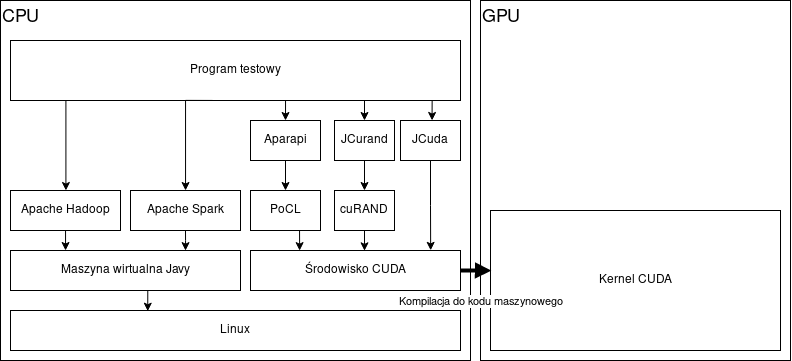
\includegraphics[width=1\textwidth]{graf/Stack.png}
	\caption{Schemat stosu oprogramowania używanego w badaniach.}
	\label{fig:software-stack}
\end{figure}

\section{Proces konfiguracji klastra}

Kluczowym elementem w budowie i ocenie wydajności klastra \english{Big Data} jest nie tylko
wybór odpowiedniego sprzętu, ale także zautomatyzowanie procesów związanych z instalacją
programów oraz konfiguracją środowiska. Zdolność do szybkiej zmiany konfiguracji pozwala na
sprawniejsze przeprowadzenie badań i dokładniejszą ocenę jego wydajności.

Wszystkie komputery zostały skonfigurowane za pomocą Ansible, czyli otwartego narzędzia
do administracji serwerami, zarządzania konfiguracją oraz wdrażania aplikacji.
\newpage

Narzędzie Ansible zostało wybrane ze względu na \cite{ansible-whitepaper}:
\begin{itemize}
	\item modułowość -- Ansible pozwala na organizację zadań w niezależne moduły
	      (nazywane też rolami), co ułatwia ponowne wykorzystanie i tworzenie złożonych zadań,
	\item idempotentność –- wielokrotne zastosowanie skryptów zawsze prowadzi do tego
	      samego stanu docelowego, zapewniając spójność konfiguracji w całym klastrze,
	\item standardowe protokoły -- Ansible komunikuje się z serwerami za pomocą
	      protokołu SSH, którego wsparcie zawarte jest w popularnych systemach operacyjnych,
	\item mechanizm inwentarzy –-  Ansible opisuje zarządzane serwery za pomocą plików w formacie
	      INI lub YAML, nazywanych też inwentarzem. W inwentarzu można tworzyć grupy złożone z
	      serwerów lub innych grup, a także zmienne przypisane do pojedynczego serwera czy grupy,
	\item mechanizm szablonów -- Ansible pozwala na generowanie plików konfiguracyjnych za pomocą
	      języka szablonów Jinja2, wspierającego użycie zmiennych, instrukcji warunkowych i pętli,
	\item wsparcie dla różnych platform –- Ansible działa na wszystkich popularnych
	      systemach operacyjnych i architekturach sprzętowych.
\end{itemize}

Ręczna część konfiguracji klastra ogranicza się do instalacji systemu operacyjnego
Jetson Linux. Po wgraniu obrazu systemu na kartę microSD i włączeniu minikomputera
uruchamiany jest instalator graficzny, w którym należy wykonać następujące czynności:
\begin{enumerate}
	\item Skonfigurować połączenie sieciowe oraz statyczny adres IP;
	\item Utworzyć konto użytkownika z hasłem;
	\item Wybrać tryb zarządzania energią "MAXN".
\end{enumerate}

Po zakończeniu pracy instalatora należy dodać statyczne adresy IP urządzeń do inwentarza
Ansible, a następnie za pomocą programu \lstinline{ansible-playbook} uruchomić kolejno
skrypty \lstinline{setup-os.yaml}, \lstinline{setup-pocl.yaml},
\lstinline{setup-hadoop.yaml} oraz \lstinline{setup-spark.yaml}.

\subsection*{Skrypty Ansible i narzędzia administracyjne}

W ramach pracy utworzono projekt Ansible, którego zadaniem jest automatyzacja procesów instalacji
programów oraz konfiguracji klastra. Skrypty Ansible wchodzące w~skład projektu zapewniają
niezawodność i powtarzalność procesów przy jednoczesnym zachowaniu czytelności
i łatwości użycia.

Kluczowym elementem każdego projektu Ansible jest inwentarz, który opisuje zbiór serwerów, na
którym mają zostać wykonane skrypty. W przypadku wspomnianego projektu inwentarz definiuje
statyczne adresy IP komputerów, podział węzłów na nadrzędne i wykonawcze, konfigurację
klienta Git, a także wersje instalowanych programów.

Kolejną częścią projektu są skrypty, które określają serię zadań do wykonania na węzłach
klastra. Zawierają one konkretne instrukcje opisane poniżej:
\begin{itemize}
	\item \lstinline{setup-os.yaml} -- przeprowadzenie wstępnej konfiguracji i aktualizacji systemu. \newline
	      Wyłączany jest tryb graficzny i ograniczenie czasu wykonania dla kerneli CUDA,
	\item \lstinline{setup-pocl.yaml} -- instalacja własnej kompilacji biblioteki PoCL,
	      dostarczającej nieoficjalne wsparcie OpenCL dla procesora graficznego w komputerze Jetson Nano,
	\item \lstinline{setup-hadoop.yaml} -- instalacja i konfiguracja platformy Apache Hadoop. \newline
	      W ramach tego skryptu formatowany jest też system plików HDFS,
	\item \lstinline{setup-spark.yaml} -- instalacja i konfiguracja platformy Apache Spark. \newline
	      W tym skrypcie instalowany jest również język programowania Scala.
\end{itemize}

Aby zwiększyć modułowość projektu, zgrupowano w role następujące zadania:
\begin{itemize}
	\item \lstinline{includes/updated} -- zadania związane z aktualizacją systemu operacyjnego,
	\item \lstinline{roles/common-tools} -- zadania do instalacji środowiska Java, konfiguracji
	      nazwy hosta, strefy czasowej oraz klienta Git,
	\item \lstinline{roles/security-config} -- konfiguracja zabezpieczeń usługi SSH.
\end{itemize}

Wykorzystując dane zawarte w inwentarzu i mechanizm szablonów udostępniany przez Ansible, skrypty
instalacyjne generują dla klastra następujące pliki konfiguracyjne:
\begin{itemize}
	\item \lstinline{core-site.xml} -- główna konfiguracja Hadoop, zawiera adres klastra HDFS,
	\item \lstinline{environment} -- konfiguracja zmiennej \lstinline{PATH}, służącej do lokalizacji programów,
	\item \lstinline{hdfs-site.xml} -- konfiguracja klastra HDFS zawierająca ustawienia replikacji danych,
	\item \lstinline{mapred-site.xml} -- konfiguracja komponentu MapReduce dla platformy Hadoop,
	\item \lstinline{yarn-site.xml} -- ustawienia menedżera zasobów YARN,
	\item \lstinline{workers} -- lista węzłów wykonawczych dla platformy Hadoop,
	\item \lstinline{spark-env.sh} -- konfiguracja platformy Spark do działania w trybie samodzielnym,
	\item \lstinline{slaves} -- lista węzłów wykonawczych dla platformy Spark.
\end{itemize}

Oprócz zadań administracyjnych, automatyzacji podlega także uruchamianie programów
testowych i zbieranie informacji o wydajności. Zapewnia to lepszą powtarzalność
pomiarów, a co za tym idzie -- większą przejrzystość i weryfikowalność badań.
Dlatego też do automatyzacji często wykonywanych zadań utworzono skrypty w języku Bash:
\begin{itemize}
	\item \lstinline{bench-*.sh} --
	      uruchamianie programów testowych dla wszystkich kombinacji
	      parametrów i danych wejściowych,
	\item \lstinline{start-hadoop.sh} i \lstinline{stop-hadoop.sh} --
	      uruchamianie i zamykanie platformy Apache Hadoop wraz z~systemem plików HDFS,
	\item \lstinline{start-spark.sh} i \lstinline{stop-spark.sh} --
	      uruchamianie i zamykanie platformy Apache Spark wraz z~systemem plików HDFS,
	\item \lstinline{clear-hdfs-out.sh} i \lstinline{clear-hdfs-tmp.sh} --
	      usuwanie plików wynikowych i plików tymczasowych programów,
	\item \lstinline{report-perf.sh} -- odczytywanie miar wydajności z
	      plików dziennika utworzonych przez programy testowe.
\end{itemize}

\section{Programy testowe}

Do badań wydajności klastra przygotowano zadania rozproszone w języku Java, które wykorzystują
platformy obliczeniowe Apache Hadoop i Apache Spark. Wszystkie programy testowe wspierają wykonanie
zarówno na procesorze głównym, jak i graficznym przy użyciu technologii CUDA. Jeden z algorytmów
został też zrealizowany przy użyciu standardu OpenCL.

Zestaw programów testowych składa się zarówno ze zmodyfikowanych wersji przykładów z dystrybucji
Hadoop oraz Spark, jak i nowych programów stworzonych na potrzeby pracy. Aby kompleksowo
ocenić wydajność klastra oraz opłacalność wykorzystania GPU w obliczeniach \english{Big Data},
zestaw testowy zawiera aplikacje o różnych charakterystykach użycia dysku i procesora.

Projekt zawierający programy testowe jest zarządzany przez Apache Maven, czyli narzędzie do
zarządzania projektami opartymi o język Java. Maven automatyzuje wiele etapów tworzenia
oprogramowania, takich jak kompilacja, testowanie, generowanie dokumentacji oraz budowanie
paczek JAR (ang. \english{Java ARchive}). Co więcej, centralne repozytorium Maven udostępnia
programistom wiele bibliotek dla języka Java, które mogą być dodawane do projektu poprzez
prostą zmianę konfiguracji.

Programy testowe zostały podzielone przy użyciu modułów Maven, czyli podprojektów wchodzących
w skład jednego projektu nadrzędnego. Moduły są kompilowane jako niezależne jednostki,
które mogą definiować zależności między sobą. Na przykład, moduł interfejsu konsolowego może
zależeć od modułu zawierającego logikę aplikacji.

Implementacje programów testowych zostały podzielone na trzy moduły:
\begin{itemize}
	\item moduł \lstinline{common} -- częściowe implementacje algorytmów w językach
	      Java oraz CUDA, funkcje ułatwiające wykonywanie programów CUDA i obsługę zasobów,
	\item moduł \lstinline{hadoop-benchmark} -- funkcje pomocnicze do zarządzania zadaniami w Apache Hadoop,
	      implementacje programów PiEstimation, FuzzyGen, FuzzyCompute oraz FuzzyFilter dla platformy Hadoop,
	\item moduł \lstinline{spark-benchmark} -- funkcje pomocnicze do zarządzania kontekstem w Apache Spark,
	      implementacje progrmaów PiEstimation, FuzzyGen, FuzzyCompute oraz FuzzyFilter dla platformy Spark.
\end{itemize}

Projekt nadrzędny może zawierać wspólną konfigurację, która może być następnie używana we
wszystkich modułach. Na przykład, zamiast określać wersje bibliotek w każdym module
osobno, można to zrobić jednokrotnie w nadrzędnym projekcie, co ułatwia aktualizację
zależności i zapewnia spójność ich wersji.

Maven posiada też wsparcie dla wtyczek, które umożliwiają dostosowywanie procesu budowy do
indywidualnych potrzeb projektu. W przypadku programów testowych wykorzystywane są wtyczki do
wykonywania narzędzia Make (wtyczka \lstinline{exec-maven-plugin}) oraz tworzenia obrazów aplikacji
wraz z wymaganymi do uruchomienia bibliotekami (wtyczka \lstinline{maven-assembly-plugin}).

\subsection{Program PiEstimation}

Pierwszym programem testowym jest PiEstimation, który wykorzystuje metodę Monte Carlo do szacowania
wartości liczby $\pi$. Wersja dla procesora głównego to rozwinięcie programu QuasiMonteCarlo
zawartego w oficjalnej dystrybucji Apache Hadoop, a jej odpowiedniki dla procesora graficznego
to autorskie konwersje w językach CUDA oraz OpenCL.

Metoda Monte Carlo to metoda numeryczna stosowana do rozwiązywania problemów poprzez próbkowanie
losowe. Oznacza to, że przeprowadzana jest symulacja wielu prób (lub "eksperymentów") w celu uzyskania
rozkładu wyników, których średnia może być następnie użyta do oszacowania oczekiwanej wartości rozwiązania.

Warianty tej metody są stosowane w wielu dziedzinach nauki, takich jak fizyka, matematyka, finanse,
czy medycyna. Jej przykładowe zastosowania to obliczanie wartości całek, szacowanie wartości
oczekiwanej, optymalizacja funkcji, symulacja sieci, symulacja zdarzeń dyskretnych i wiele innych.

Szacowanie liczby $\pi$ za pomocą metody Monte Carlo to klasyczny przykład zastosowania tej techniki.
Wykonuje się w nim losowe próbkowanie punktów wewnątrz kwadratu i określa ich położenie względem
wpisanego w ten kwadrat koła, co ilustruje rysunek \ref{fig:monte-carlo}.

\begin{figure}[h]
	\centering
	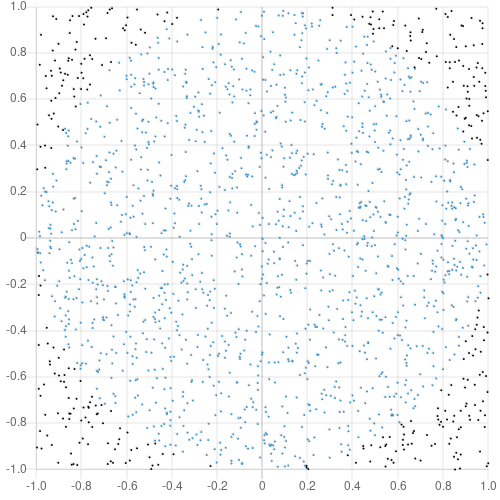
\includegraphics[width=0.8\textwidth]{graf/Pi-estimation.png}
	\caption{Rozkład wartości losowych używany do estymacji liczby $\pi$.}
	\medskip \small
	Czarne punkty znajdują się poza kołem, a punkty niebieskie -- wewnątrz koła.
	\label{fig:monte-carlo}
\end{figure}

\subsubsection*{Implementacja metody Monte Carlo}

Rozważmy kwadrat o boku długości 2, którego środek znajduje się w punkcie (0,0). W ten kwadrat wpisywane
jest koło o promieniu 1, również o środku w punkcie (0,0). Powierzchnia kwadratu wynosi więc 4, a
powierzchnia koła jest równa $\pi$.

Następnie wybieramy losowo punkty o losowych współrzędnych X i Y z zakresu [-1, 1], czyli znajdujących
się wewnątrz kwadratu. Dla każdego punktu sprawdzamy, czy leży on wewnątrz koła. Robimy to, obliczając
jego odległość od środka kwadratu (i koła) za pomocą wzoru \(d = x^2 + y^2\). Jeśli odległość
jest mniejsza lub równa 1, punkt leży wewnątrz koła, a w przeciwnym razie leży poza nim.

Po przeprowadzeniu wielu takich prób obliczamy stosunek liczby punktów wewnątrz koła do
całkowitej liczby punktów wewnątrz kwadratu. Wraz ze zwiększającą się liczbą wybranych
punktów stosunek punktów wewnątrz okręgu do punktów wewnątrz kwadratu będzie coraz
bardziej zbliżony do stosunku ich powierzchni, czyli \(\pi / 4\).

Programy komputerowe realizujące metodę Monte Carlo najczęściej używają generatora liczb
pseudolosowych, którego jakość, wraz z liczbą wybranych punktów, jest głównym czynnikiem
wpływającym na dokładność wyniku.

Użyty w programie generator liczb pseudolosowych oparty jest o ciąg Haltona, czyli
technikę generowania ciągów opartą o rozwinięcia w systemach liczbowych o różnych podstawach.
W przeciwieństwie do tradycyjnych sekwencji losowych sekwencje te zapewniają bardziej
jednolite próbkowanie przestrzeni, co ogranicza błąd obliczeń \cite{monte-carlo}.

Algorytm generacji punktów z użyciem sekwencji Haltona jest nastepujący:
\begin{enumerate}
	\item Dla każdego wymiaru wybierz unikalną liczbę pierwszą \( p \),
	\item Dla każdej liczby pierwszej \( p \) i kolejnych liczb \( i \),
	      wygeneruj rozwinięcia liczb \( i \) o~podstawie \( p \),
	\item Przekształć rozwinięcia liczb \( i \) na wartość ułamkową, aby uzyskać
	      elementy sekwencji dla tej podstawy,
	\item Połącz powstałe sekwencje w celu uzyskania wielowymiarowych punktów.
\end{enumerate}

Ponieważ wartości generowane przez sekwencję są stałe i zależą tylko od podstaw sekwencji,
testowanie implementacji w różnych językach sprowadzało się do porównania końcowych wyników.

Program dla platformy Hadoop wykorzystuje następujące komponenty \english{Mapper},
które zostały opisane w załączniku \ref{ch:techdoc}:
\begin{itemize}
	\item CpuQmcMapper (listing \ref{ch:cpu-qmc-mapper}) -- implementacja dla procesora głównego,
	\item AparapiQmcMapper (listing \ref{ch:aparapi-qmc-mapper}) -- implementacja w języku Java wykorzystująca bibliotekę Aparapi i OpenCL,
	\item JcudaQmcMapper (listing \ref{ch:jcuda-qmc-mapper}) -- implementacja algorytmu w języku CUDA.
\end{itemize}

Ich odpowiednikami dla platformy Spark są klasy CpuQmcFunction, AparapiQmcFunction oraz JcudaQmcFunction (listingi \ref{ch:cpu-qmc-function}, \ref{ch:aparapi-qmc-function} oraz
\ref{ch:jcuda-qmc-function}).

\subsubsection*{Specyfikacja zewnętrzna}

Programy dla platform Apache Hadoop oraz Apache Spark oczekują trzech argumentów wiersza poleceń:
\begin{itemize}
	\item \lstinline{nMaps} -- liczba niezależnych zadań używanych w estymacji,
	\item \lstinline{nSamples} -- liczba próbek przetwarzanych w jednym zadaniu,
	\item \lstinline{mapper} -- implementacja algorytmu (jedna z wartości "cpu", "opencl" lub "cuda").
\end{itemize}

Program wyświetla w konsoli liczbę próbek, algorytm, czas wykonania oraz oszacowaną wartość liczby $\pi$, co przedstawiono na rysunku \ref{fig:piestimation:run}.
Jeśli argumenty nie zostały dostarczone lub są nieprawidłowe, aplikacja wyświetli komunikat o
błędzie wraz z instrukcją poprawnego użycia.

\begin{figure}[h]
	\centering
	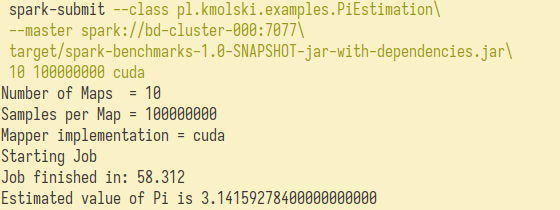
\includegraphics[width=0.8\textwidth]{graf/PiEstimation-interface.png}
	\caption{Przykładowe wywołanie programu PiEstimation.}
	\label{fig:piestimation:run}
\end{figure}

Aplikacja dla platformy Hadoop zapisuje pliki tymczasowe w katalogach \lstinline{/tmp} i \lstinline{/out}
systemu plików HDFS, które są usuwane po zakończeniu zadania.

\subsection{Program FuzzyGen}

Zadaniem kolejnego programu testowego jest generowanie zbiorów danych o różnej objętości dla programu
FuzzyCompute. Dane programu FuzzyCompute składają się z~wielu porcji, z~których każda zawiera 64
zbiory. Każdy zbiór zawiera stopnie przynależności dla 4 rekordów, w~zakresie od 0 do 1.

Porcje danych są zapisywane jako pliki binarne w formacie SequenceFile, dostarczanym przez platformę
Hadoop. Pliki SequenceFile przechowują pary klucz-wartość w skompresowanej formie, co pozwala
zmniejszyć zapotrzebowanie na przestrzeń dyskową i~zwiększyć efektywną szybkość systemu plików.

Algorytm dla procesora głównego wykorzystuje generator liczb losowych z biblioteki standardowej języka Java,
który jest oparty o liniowe generatory kongruentne. Generator ten jest oparty o deterministyczny algorytm i
zapewnia stosunkowo dobrą wydajność, nie jest jednak odpowiedni do zastosowań kryptograficznych.

Wersja algorytmu dla procesora graficznego wykorzystuje bibliotekę JCurand, która udostępnia
funkcjonalność biblioteki cuRAND w języku Java. Biblioteka cuRAND jest z kolei częścią zestawu narzędzi
deweloperskich CUDA, dostarczającą funkcje do generowania liczb losowych na procesorach graficznych
firmy NVIDIA.
\newpage

cuRAND oferuje kilka typów generatorów liczb pseudolosowych, są to między innymi:
\begin{itemize}
	\item generator XORWOW,
	\item generator MRG32K3A,
	\item generator Mersenne Twister (MT19937),
	\item generator Philox 4x32.
\end{itemize}

Za pomocą generatorów cuRAND możliwe jest generowanie liczb dla różnych rozkładów prawdopodobieństwa,
takich jak rozkład Poissona, jednostajny lub normalny.

Program Hadoop wykorzystuje następujące klasy komponentów \english{Mapper},
które zostały opisane w załączniku \ref{ch:techdoc}:
\begin{itemize}
	\item CpuFuzzyGenMapper (listing \ref{ch:cpu-fuzzygen-mapper}) -- algorytm dla procesora głównego,
	\item JcudaFuzzyGenMapper (listing \ref{ch:jcuda-fuzzygen-mapper}) -- algorytm używający funkcji z biblioteki JCurand.
\end{itemize}

W programie dla Apache Spark wykorzystywane są klasy CpuFuzzyGenFunction i~JcudaFuzzyGenFunction (listingi \ref{ch:cpu-fuzzygen-function} oraz \ref{ch:jcuda-fuzzygen-function}).

\subsubsection*{Specyfikacja zewnętrzna}

Aplikacje dla Apache Hadoop oraz Apache Spark oczekują trzech argumentów wiersza poleceń:
\begin{itemize}
	\item \lstinline{mapper} -- definiujący wykorzystywany algorytm (do wyboru: "cpu" lub "cuda"),
	\item \lstinline{nRecords} -- liczba porcji danych do wygenerowania,
	\item \lstinline{outputDir} -- katalog HDFS, w którym zostaną zapisane pliki wynikowe.
\end{itemize}

Program wyświetla w konsoli liczbę porcji danych, algorytm oraz czas wykonania, co przedstawiono
na rysunku \ref{fig:fuzzygen:run}. Gdy wymagane argumenty nie zostaną podane lub są błędne,
program pokazuje komunikat o~błędzie oraz instrukcję prawidłowego użycia.

\begin{figure}[h]
	\centering
	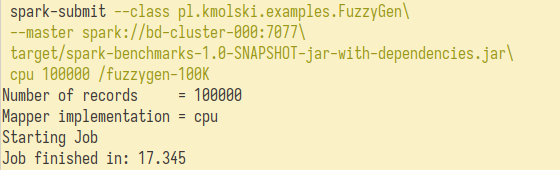
\includegraphics[width=0.8\textwidth]{graf/FuzzyGen-interface.png}
	\caption{Przykładowe wywołanie programu FuzzyGen.}
	\label{fig:fuzzygen:run}
\end{figure}

Zarówno program dla platformy Hadoop, jak i~odpowiednik dla platformy Spark zapisuje dane
wyjściowe w formacie SequenceFile bez użycia kompresji. Zadanie Hadoop definiuje tylko
etap \english{Map}, przez co pliki wynikowe są zapisywane w kilku częściach.

\subsection{Program FuzzyCompute}

Kolejny program jest testem wydajności dla operacji wykonywanych na zbiorach rozmytych.
Zbiory rozmyte stanowią centralny element logiki rozmytej i zostały zdefiniowane przez
Lotfi Zadeha jako rozwinięcie tradycyjnej teorii zbiorów. Umożliwiają one reprezentację
niejasności i wieloznaczności w klasyfikacji obiektów \cite{fuzzy-sets}.

Zbiory rozmyte znalazły szerokie zastosowanie w różnych dziedzinach, takich jak sterowanie
rozmyte, systemy ekspertowe, analiza ryzyka oraz przetwarzanie obrazów. Znacząco ułatwiają
one modelowanie sytuacji, w których granice decyzyjne są trudne do określenia.

W klasycznej teorii zbiorów element albo należy do zbioru (i ma przynależność równą 1),
albo do niego nie należy (i ma przynależność równą 0). W zbiorach rozmytych stopień
przynależności elementu jest opisany przez funkcję przynależności, która przyjmuje wartość
liczbową w zakresie od 0 do 1.

Rozważmy zbiór przedmiotów pochodzących z różnych epok. Używając klasycznej teorii zbiorów,
możemy określić jedynie to, że dany przedmiot albo jest antykiem, albo nim nie jest. Jeśli
wiek przedmiotu znajdzie się tuż pod przyjętym progiem, to zostanie sklasyfikowany jako nie-antyk.

Jeżeli jednak opiszemy te same przedmioty za pomocą zbiorów rozmytych, możemy uzyskać bardziej
użyteczną klasyfikację. Przykładowo, funkcja przedstawiona na rysunku \ref{fig:fuzzy-fn} przypisuje
20-letni przedmiot do zbioru antyków z przynależnością 0, 250-letni -- z~przynależnością 0.5, a
500-letni -- z przynależnością wynoszącą 1.

\begin{figure}[h]
	\centering
	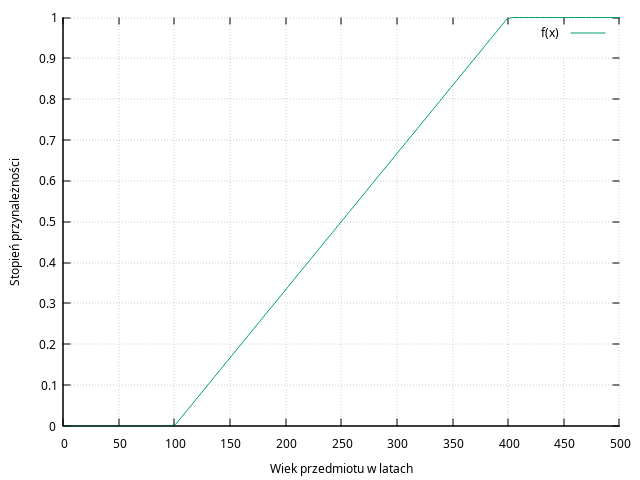
\includegraphics[width=0.6\textwidth]{graf/Fuzzy-membership.png}
	\caption{Wykres przykładowej funkcji przynależności dla zbioru rozmytego.}
	\label{fig:fuzzy-fn}
\end{figure}

Podobnie jak w klasycznej teorii zbiorów, na zbiorach rozmytych definiowane są różne operacje,
takie jak suma, iloczyn, czy dopełnienie. Podczas gdy koncepcja tych operacji pozostaje podobna,
ich realizacje różnią się od tych znanych z klasycznej teorii zbiorów, ponieważ uwzględniają
rozmyte podejście do przynależności.

Suma zbiorów rozmytych może być zdefiniowana jako maksimum stopni przynależności każdego elementu do
obu zbiorów. Niech \(A\) i \(B\) będą zbiorami rozmytymi w przestrzeni \(X\) z funkcjami
przynależności odpowiednio \(\mu A\) i \(\mu B\). Suma zbiorów \(A\) i \(B\) jest zbiorem rozmytym
\(C\) z funkcją przynależności \(\mu C\), która jest definiowana następująco dla każdego elementu
w przestrzeni \(X\) za pomocą wzoru \ref{eq:fuzzy-sum}.

\begin{equation}
    \mu C(x) = max(\mu A(x), \mu B(x))
    \label{eq:fuzzy-sum}
\end{equation}

Dla każdego elementu \(x\) stopień przynależności do sumy \(C\) jest większym z dwóch stopni
przynależności do zbiorów \(A\) i \(B\). Taką operację binarną, używaną do modelowania operacji
"lub" w kontekście zbiorów rozmytych, nazywamy T-konormą lub S-normą. Do S-norm można zaliczyć
też sumę algebraiczną, sumę drastyczną, czy sumę Łukasiewicza.

Dopełnienie zbioru rozmytego polega na odwróceniu stopnia przynależności każdego elementu w
danym zbiorze rozmytym. Jeśli mamy zbiór rozmyty \(A\) na przestrzeni uniwersalnej \(X\) z
funkcją przynależności \(\mu A\), dopełnienie tego zbioru, oznaczone jako \(A'\) lub \(\lnot A\),
ma funkcję przynależności \(\mu A'\) określoną dla każdego elementu \(x\) z \(X\)
wzorem \ref{eq:fuzzy-compl}.

\begin{equation}
    \mu A'(x) = 1 - \mu A(x)
    \label{eq:fuzzy-compl}
\end{equation}

Aplikacje dla platform Hadoop oraz Spark przetwarzają podziały zbiorów wygenerowanych przez program
FuzzyGen. Składają się one z 64 zbiorów, z~których każdy zawiera cztery liczby losowe z~zakresu od
0 do 1. Po wczytaniu zbiorów rozmytych, do zbioru danych dodawane są ich dopełnienia.
Następnie wszystkie zbiory rozmyte są sumowane krzyżowo, co zwiększa złożoność obliczeniową programu.

Aplikacja dla platformy Hadoop wykorzystuje następujące komponenty \english{Mapper},
które zostały opisane w załączniku \ref{ch:techdoc}:
\begin{itemize}
	\item CpuFuzzyComputeMapper (listing \ref{ch:cpu-fuzzycompute-mapper}) -- algorytm dla procesora głównego,
	\item JcudaFuzzyComputeMapper (listing \ref{ch:jcuda-fuzzycompute-mapper}) -- algorytm używający kerneli w języku CUDA.
\end{itemize}

Ich odpowiednikami dla programu Apache Spark są klasy CpuFuzzyComputeFunction i JcudaFuzzyComputeFunction (listingi \ref{ch:cpu-fuzzycompute-function} oraz \ref{ch:jcuda-fuzzycompute-function}).

\subsubsection*{Specyfikacja zewnętrzna}

Dla programów opartych o Apache Hadoop i Apache Spark konieczne jest podanie trzech parametrów wiersza poleceń, które zostały również przedstawione na rysunku \ref{fig:fuzzycompute:run}:
\begin{itemize}
	\item \lstinline{mapper} -- określający typ algorytmu (do wyboru "cpu" lub "cuda"),
	\item \lstinline{inputDir} -- katalog HDFS z plikami wejściowymi,
	\item \lstinline{outputDir} -- katalog HDFS, w którym zostanie zapisany wynik działania programu.
\end{itemize}

Program prezentuje w konsoli wykorzystywany algorytm oraz czas jego działania. W~przypadku podania
nieprawidłowych parametrów program poinformuje o~błędzie i~przedstawi poprawną składnię parametrów.

\begin{figure}[h]
	\centering
	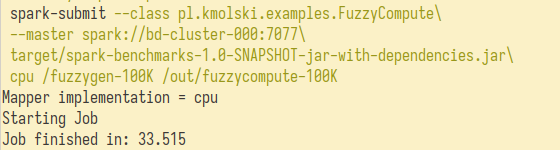
\includegraphics[width=0.8\textwidth]{graf/FuzzyCompute-interface.png}
	\caption{Przykładowe wywołanie programu FuzzyCompute.}
	\label{fig:fuzzycompute:run}
\end{figure}

Formatem plików wejściowych i wyjściowych dla programu jest SequenceFile.

\subsection{Program FuzzyFilter}

Ostatni z omawianych programów testowych implementuje filtrowanie rekordów z plików CSV przy użyciu
zbiorów rozmytych. Filtrowanie danych z użyciem zbiorów rozmytych polega na zastosowaniu logiki
rozmytej do określenia stopnia przynależności elementów, a następnie usunięciu rekordów, których
stopień przynależności znajduje się poniżej ustawionego progu.

Tradycyjne metody klasyfikacji przyjmują, że obiekt należy do jednej konkretnej klasy. W podejściu
opartym na zbiorach rozmytych obiekt może należeć do wielu klas jednocześnie z różnym stopniem
przynależności. Pozwala to na lepsze uwzględnienie niepewności i niejednoznaczności w danych,
dzięki czemu klasyfikacja jest bardziej elastyczna i lepiej odwzorowuje rzeczywistość.

Funkcje przynależności dla zbiorów rozmytych mogą przyjmować różne kształty, które pozwalają na opisanie
stopnia przynależności w zależności od charakteru danych i problemu. Oto kilka najpopularniejszych
typów funkcji przynależności \cite{fuzzy-sets}:
\begin{itemize}
	\item funkcja impulsowa -- funkcja ta ma wartość 1 dla konkretnego punktu w zbiorze uniwersalnym i
	      0 dla wszystkich innych punktów,
	\item funkcja trójkątna -- określona przez trzy punkty: punkt początkowy, punkt szczytowy i
	      punkt końcowy. Wartość funkcji przynależności wzrasta liniowo od punktu początkowego do punktu
	      szczytowego, a następnie maleje liniowo do punktu końcowego,
	\item funkcja trapezoidalna -- podobna do funkcji trójkątnej, ale z dodatkowym płaskim segmentem dla
	      wartości 1. Zdefiniowana jest przez cztery punkty: punkt początkowy, punkt początku segmentu
	      płaskiego, punkt końca segmentu płaskiego i punkt końcowy,
	\item funkcja Gaussa -- funkcja dzwonowa zdefiniowana przez średnią i odchylenie standardowe.
	      Pozwala na modelowanie stopniowej przynależności, która jest maksymalna w środku i maleje w
	      kierunku wartości krańcowych.
\end{itemize}

Program pozwala na definiowanie relacji przynależności na podstawie funkcji trapezoidalnej. Zaletą tej
funkcji jest jej elastyczność w modelowaniu różnych relacji przynależności. W zależności od wybranych punktów,
określających kształt trapezu, można osiągnąć różne kształty funkcji przynależności.

Ponieważ funkcja trójkątna jest specyficznym przypadkiem funkcji trapezoidalnej, użytkownik może zdefiniować
ją poprzez podanie takich samych wartości dla obu punktów definiujących segment płaski trapezu. Podobne
rozwiązanie umożliwia określenie funkcji impulsowej. Podanie tej samej wartości dla wszystkich parametrów
trapezu powoduje, że powstała funkcja przyjmuje wartość 1 tylko dla jednego punktu.

Podana przez użytkownika lista trapezoidalnych funkcji przynależności jest łączona za pomocą T-normy,
która reprezentuje operację koniunkcji w~dziedzinie zbiorów rozmytych. Przykładowe T-normy to minimum,
produkt algebraiczny oraz norma Łukasiewicza. W programie wykorzystano najprostszą z~nich, czyli
T-normę minimum, która dla dwóch stopni przynależności \( a \) i \( b \) z~zakresu [0, 1] jest
określana przez wzór \ref{eq:fuzzy-tnorm}.

\begin{equation}
    T_{\text{min}}(a, b) = \min(a, b)
    \label{eq:fuzzy-tnorm}
\end{equation}

T-norma minimum ma następujące właściwości:
\begin{itemize}
    \item monotoniczność -- minimum jest funkcją monotoniczną. Oznacza to, że jeżeli mamy dwie pary liczb,
          gdzie \( a \leq c \) i \( b \leq d \), to zawsze \( T_{\text{min}}(a, b) \leq T_{\text{min}}(c, d) \),
    \item idempotentność -- T-norma minimum jest idempotentna, co w praktyce oznacza, że \( T_{\text{min}}(a, a) \)
          zawsze równa się \( a \) dla dowolnej liczby \( a \),
    \item element neutralny --  dla funkcji minimum elementem neutralnym jest liczba 1. Innymi słowy,
          \( T_{\text{min}}(a, 1) \) zawsze równa się \( a \) dla dowolnego \( a \) z przedziału [0, 1],
    \item komutatywność -- oznacza to, że funkcja minimum zwraca ten sam wynik niezależnie od kolejności
          argumentów, czyli \( T_{\text{min}}(a, b) \) jest równa \( T_{\text{min}}(b, a) \)
          dla dowolnych liczb \( a \) i \( b \),
    \item łączność -- funkcja minimum jest również łączna. W praktyce oznacza to, że dla dowolnych
          liczb \( a \), \( b \) i \( c \) z przedziału [0, 1], \( T_{\text{min}}(a, T_{\text{min}}(b, c)) \)
          jest równa \( T_{\text{min}}(T_{\text{min}}(a, b), c) \).
\end{itemize}

Program dla platformy Spark wykorzystuje moduł Spark SQL, który został wybrany ze względu na zdolność
do operowania na plikach CSV bez definiowania schematu danych. Umożliwia to przetwarzanie danych o różnej
strukturze bez konieczności zmiany programu. Rozmyte filtrowanie rekordów jest implementowane przez klasy opisane w załączniku \ref{ch:techdoc}:
\begin{itemize}
    \item CpuFuzzyFilterFunction (listing \ref{ch:cpu-fuzzyfilter-function}) -- implementacja dla procesora głównego,
    \item JcudaFuzzyFilterFunction (listing \ref{ch:jcuda-fuzzyfilter-function}) -- implementacja używająca algorytmu w języku CUDA.
\end{itemize}

\subsubsection*{Specyfikacja zewnętrzna}

Program Spark oczekuje co najmniej czterech argumentów wiersza poleceń, których przykładowe użycie
zostało przedstawione na rysunku \ref{fig:fuzzyfilter:run}:
\begin{itemize}
	\item \lstinline{mapper} -- implementacja algorytmu (jeden z "cpu" lub "cuda"),
	\item \lstinline{inputFile} -- plik wejściowy w formacie CSV,
	\item \lstinline{outputFile} -- ścieżka pliku w HDFS, do którego zostaną zapisane rekordy,
	\item \lstinline{threshold} -- wartość progowa dla funkcji przynależności rekordu,
    \item \lstinline{filters} -- parametry określające trapezoidalną funkcję przynależności.
\end{itemize}

Składnia parametru \lstinline{filters} składa się z pięciu części:
\begin{itemize}
	\item punktu początkowego,
	\item punktu początku segmentu płaskiego,
	\item punktu końca segmentu płaskiego,
	\item punktu końcowego,
    \item kolumny, dla której obliczany jest stopień przynależności
\end{itemize}

Program wyświetla w konsoli wybrany algorytm, czas wykonania oraz liczbę rekordów spełniających
zadany warunek. W przypadku braku argumentów lub ich niepoprawności, aplikacja poinformuje użytkownika
o~błędzie i~przedstawi instrukcję właściwego użycia.

\begin{figure}[h]
	\centering
	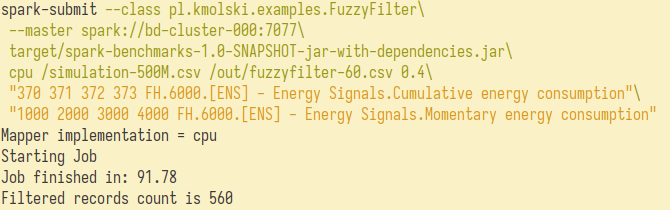
\includegraphics[width=0.8\textwidth]{graf/FuzzyFilter-interface.png}
	\caption{Przykładowe wywołanie programu FuzzyFilter.}
	\label{fig:fuzzyfilter:run}
\end{figure}

Format plików odczytywanych i~zapisywanych przez program FuzzyFilter to CSV.
 % [Przedmiot pracy]
\chapter{Badania}
%
% 
%
%Rozdział przedstawia przeprowadzone badania. Jest to zasadnicza część i~musi wyraźnie dominować w~pracy.
%Badania i analizę wyników należy przeprowadzić, tak jak jest przyjęte w środowisku naukowym (na przykład korzystanie z danych benchmarkowych, walidacja krzyżowa, zapewnienie powtarzalności testów itd). 
%
%\section{Metodyka badań}
%
%\begin{itemize}
%\item opis metodyki badań
%\item opis stanowiska badawczego (opis interfejsu aplikacji badawczych -- w~załączniku)
%\end{itemize}
%
%
%\section{Zbiory danych}
%
%\begin{itemize}
%\item opis danych
%\end{itemize}
%
%
%\section{Wyniki}
%
%\begin{itemize}
%\item prezentacja wyników, opracowanie i poszerzona dyskusja  wyników, wnioski
%\end{itemize}
%
% 
%\begin{table}
%\centering
%\caption{Opis tabeli nad nią.}
%\label{id:tab:wyniki}
%\begin{tabular}{rrrrrrrr}
%\toprule
%	         &                                     \multicolumn{7}{c}{metoda}                                      \\
%	         \cmidrule{2-8}
%	         &         &         &        \multicolumn{3}{c}{alg. 3}        & \multicolumn{2}{c}{alg. 4, $\gamma = 2$} \\
%	         \cmidrule(r){4-6}\cmidrule(r){7-8}
%	$\zeta$ &     alg. 1 &   alg. 2 & $\alpha= 1.5$ & $\alpha= 2$ & $\alpha= 3$ &   $\beta = 0.1$  &   $\beta = -0.1$ \\
%\midrule
%	       0 &  8.3250 & 1.45305 &       7.5791 &    14.8517 &    20.0028 & 1.16396 &                       1.1365 \\
%	       5 &  0.6111 & 2.27126 &       6.9952 &    13.8560 &    18.6064 & 1.18659 &                       1.1630 \\
%	      10 & 11.6126 & 2.69218 &       6.2520 &    12.5202 &    16.8278 & 1.23180 &                       1.2045 \\
%	      15 &  0.5665 & 2.95046 &       5.7753 &    11.4588 &    15.4837 & 1.25131 &                       1.2614 \\
%	      20 & 15.8728 & 3.07225 &       5.3071 &    10.3935 &    13.8738 & 1.25307 &                       1.2217 \\
%	      25 &  0.9791 & 3.19034 &       5.4575 &     9.9533 &    13.0721 & 1.27104 &                       1.2640 \\
%	      30 &  2.0228 & 3.27474 &       5.7461 &     9.7164 &    12.2637 & 1.33404 &                       1.3209 \\
%	      35 & 13.4210 & 3.36086 &       6.6735 &    10.0442 &    12.0270 & 1.35385 &                       1.3059 \\
%	      40 & 13.2226 & 3.36420 &       7.7248 &    10.4495 &    12.0379 & 1.34919 &                       1.2768 \\
%	      45 & 12.8445 & 3.47436 &       8.5539 &    10.8552 &    12.2773 & 1.42303 &                       1.4362 \\
%	      50 & 12.9245 & 3.58228 &       9.2702 &    11.2183 &    12.3990 & 1.40922 &                       1.3724 \\
%\bottomrule
%\end{tabular}
%\end{table}  
%
%
% 
%\begin{figure}
%\centering
%\begin{tikzpicture}
%\begin{axis}[
%    y tick label style={
%        /pgf/number format/.cd,
%            fixed,   % po zakomentowaniu os rzednych jest indeksowana wykladniczo
%            fixed zerofill, % 1.0 zamiast 1
%            precision=1,
%        /tikz/.cd
%    },
%    x tick label style={
%        /pgf/number format/.cd,
%            fixed,
%            fixed zerofill,
%            precision=2,
%        /tikz/.cd
%    }
%]
%\addplot [domain=0.0:0.1] {rnd};
%\end{axis} 
%\end{tikzpicture}
%\caption{Podpis rysunku po rysunkiem.}
%\label{fig:2}
%\end{figure}
%
%
%\begin{figure}
%\begin{lstlisting}
%if (_nClusters < 1)
%	throw std::string ("unknown number of clusters");
%if (_nIterations < 1 and _epsilon < 0)
%	throw std::string ("You should set a maximal number of iteration or minimal difference -- epsilon.");
%if (_nIterations > 0 and _epsilon > 0)
%	throw std::string ("Both number of iterations and minimal epsilon set -- you should set either number of iterations or minimal epsilon.");
%\end{lstlisting}
%\caption{Przykład pseudokodu}
%\end{figure}
 % Badania

\chapter{Podsumowanie}

%\begin{itemize}
%\item Jaki problem rozwiązałæm?
%\item Jak ten problem rozwiązałæm?
%\item Jakie są dobre i słabe strony mojego rozwiązania?
%\item Czy mogę sformułować jakieś rekomendacje?
%\end{itemize}

\begin{itemize}
\item syntetyczny opis wykonanych prac
\item wnioski
\item możliwość rozwoju, kontynuacji prac, potencjalne nowe kierunki
\item Czy cel pracy zrealizowany? 
\end{itemize}

 % Podsumowanie

\backmatter

%\bibliographystyle{plplain}  % bibtex
%\bibliography{biblio/biblio} % bibtex
\printbibliography           % biblatex
\addcontentsline{toc}{chapter}{Bibliografia}

\begin{appendices}

    
 % dokumentacja techniczna
    \chapter{Spis skrótów i symboli}

\begin{itemize}
    \item[SoC] -- system na czipie (ang. \english{system on a chip}),
    \item[GPGPU] -- obliczenia ogólnego przeznaczenia na układach graficznych (ang. \english{General-Purpose Compute on Graphics Processing Units}),
    \item[SBC] -- komputer jednopłytkowy (ang. \english{single-board computer}),
    \item[SMP] -- wieloprocesorowość symetryczna (ang. \english{Symmetric Multiprocessing}),
    \item[HDFS] -- rozproszony system plików Hadoop (ang. \english{Hadoop Distributed File System}),
    \item[SIMD] -- jedna instrukcja, wiele danych (ang. \english{Single Instruction, Multiple Data}),
    \item[SIMT] -- jedna instrukcja, wiele wątków (ang. \english{Single Instruction, Multiple Threads}).
\end{itemize} % Spis skrótów i symboli
    \chapter{Lista dodatkowych plików, uzupełniających tekst pracy (jeżeli dotyczy)} 

W systemie do pracy dołączono dodatkowe pliki zawierające:
\begin{itemize}
\item źródła programu,
\item zbiory danych użyte w~eksperymentach,
\item film pokazujący działanie opracowanego oprogramowania lub zaprojektowanego i wykonanego urządzenia,
\item itp.
\end{itemize}
 % Lista dodatkowych plików

    \listoffigures
    \addcontentsline{toc}{chapter}{Spis rysunków}
    \listoftables
    \addcontentsline{toc}{chapter}{Spis tabel}

\end{appendices}

\end{document}


%% Finis coronat opus.

